\documentclass[11pt,a4paper]{report}%especifica o tipo de documento que tenciona escrever: carta, artigo, relatório... neste caso é um relatório
% [11pt,a4paper] Define o tamanho principal das letras do documento. caso não especifique uma delas, é assumido 10pt
% a4paper -- Define o tamanho do papel.
\usepackage{tabularx}
\usepackage{float}
\usepackage[portuges]{babel}%Babel -- irá activar automaticamente as regras apropriadas de hifenização para a língua todo o
                                   %-- o texto gerado é automaticamente traduzido para Português.
                                   %  Por exemplo, “chapter” irá passar a “capítulo”, “table of contents” a “conteúdo”.
                                   % portuges -- específica para o Português.
\usepackage[utf8]{inputenc} % define o encoding usado texto fonte (input)--usual "utf8" ou "latin1

\usepackage{graphicx} %permite incluir graficos, tabelas, figuras
\usepackage{url} % para utilizar o comando \url{}
\usepackage{enumerate} %permite escolher, nas listas enumeradas, se os iems sao marcados com letras ou numeros-romanos em vez de numeracao normal

%\usepackage{apalike} % gerar biliografia no estilo 'named' (apalike)

\usepackage{color} % Para escrever em cores

\usepackage{multirow} %tabelas com multilinhas
\usepackage{array} %formatação especial de tabelas em array

\usepackage[pdftex]{hyperref} % transformar as referências internas do seu documento em hiper-ligações.

%Exemplos de fontes -- nao e vulgar mudar o tipo de fonte
%\usepackage{tgbonum} % Fonte de letra: TEX Gyre Bonum
%\usepackage{lmodern} % Fonte de letra: Latin Modern Sans Serif
%\usepackage{helvet}  % Fonte de letra: Helvetica
%\usepackage{charter} % Fonte de letra:Charter

\definecolor{saddlebrown}{rgb}{0.55, 0.27, 0.07} % para definir uma nova cor, neste caso 'saddlebrown'

\usepackage{listings}  % para utilizar blocos de texto verbatim no estilo 'listings'
%paramerização mais vulgar dos blocos LISTING - GENERAL
\lstset{
	basicstyle=\small, %o tamanho das fontes que são usadas para o código
	numbers=left, % onde colocar a numeração da linha
	numberstyle=\tiny, %o tamanho das fontes que são usadas para a numeração da linha
	numbersep=5pt, %distancia entre a numeração da linha e o codigo
	breaklines=true, %define quebra automática de linha
    frame=tB,  % caixa a volta do codigo
	mathescape=true, %habilita o modo matemático
	escapeinside={(*@}{@*)} % se escrever isto  aceita tudo o que esta dentro das marcas e nao altera
}
%
%\lstset{ %
%	language=Java,							% choose the language of the code
%	basicstyle=\ttfamily\footnotesize,		% the size of the fonts that are used for the code
%	keywordstyle=\bfseries,					% set the keyword style
%	%numbers=left,							% where to put the line-numbers
%	numberstyle=\scriptsize,				% the size of the fonts that are used for the line-numbers
%	stepnumber=2,							% the step between two line-numbers. If it's 1 each line
%											% will be numbered
%	numbersep=5pt,							% how far the line-numbers are from the code
%	backgroundcolor=\color{white},			% choose the background color. You must add \usepackage{color}
%	showspaces=false,						% show spaces adding particular underscores
%	showstringspaces=false,					% underline spaces within strings
%	showtabs=false,							% show tabs within strings adding particular underscores
%	frame=none,								% adds a frame around the code
%	%abovecaptionskip=-.8em,
%	%belowcaptionskip=.7em,
%	tabsize=2,								% sets default tabsize to 2 spaces
%	captionpos=b,							% sets the caption-position to bottom
%	breaklines=true,						% sets automatic line breaking
%	breakatwhitespace=false,				% sets if automatic breaks should only happen at whitespace
%	title=\lstname,							% show the filename of files included with \lstinputlisting;
%											% also try caption instead of title
%	escapeinside={\%*}{*)},					% if you want to add a comment within your code
%	morekeywords={*,...}					% if you want to add more keywords to the set
%}

\usepackage{xspace} % deteta se a seguir a palavra tem uma palavra ou um sinal de pontuaçao se tiver uma palavra da espaço, se for um sinal de pontuaçao nao da espaço

\parindent=0pt %espaço a deixar para fazer a  indentação da primeira linha após um parágrafo
\parskip=2pt % espaço entre o parágrafo e o texto anterior

\setlength{\oddsidemargin}{-1cm} %espaço entre o texto e a margem
\setlength{\textwidth}{18cm} %Comprimento do texto na pagina
\setlength{\headsep}{-1cm} %espaço entre o texto e o cabeçalho
\setlength{\textheight}{23cm} %altura do texto na pagina

% comando '\def' usado para definir abreviatura (macros)
% o primeiro argumento é o nome do novo comando e o segundo entre chavetas é o texto original, ou sequência de controle, para que expande
\def\darius{\textsf{Darius}\xspace}
\def\antlr{\texttt{AnTLR}\xspace}
\def\pe{\emph{Publicação Eletrónica}\xspace}
\def\titulo#1{\section{#1}}    %no corpo do documento usa-se na forma '\titulo{MEU TITULO}'
\def\super#1{{\em Supervisor: #1}\\ }
\def\area#1{{\em \'{A}rea: #1}\\[0.2cm]}
\def\resumo{\underline{Resumo}:\\ }

%\input{LPgeneralDefintions} %permite ler de um ficheiro de texto externo mais definições

\title{Projeto de Engenharia de Requisitos\\
        1º/4º ano MEI/MIEI\\
       \textbf{Projeto ShareCar}\\ Documento de Requisitos
       } %Titulo do documento
%\title{Um Exemplo de Artigo em \LaTeX}
\author{Isaac Paulo Betuel Mabiala\\ (pg41074@alunos.uminho.pt) \and Rapahel Pinheiro \\ (pg37160@alunos.uminho.pt) \and José André Martins Pereira\\ (a82880@alunos.uminho.pt) \and Ricardo André Gomes Petronilho\\ (a81744@alunos.uminho.pt)
       } %autores do documento
\date{\today} %data

\begin{document} % corpo do documento

\begin{figure}
    \centering
    
\includegraphics{imagens/uminho.png}
\end{figure}

\maketitle % apresentar titulo, autor e data

\tableofcontents % Insere a tabela de indice
%\listoffigures % Insere a tabela de indice figuras
%\listoftables % Insere a tabela de indice tabelas

\chapter{O propósito do projeto}

\section{Contextualização}

Cada vez mais percebe-se um aumento na quantidade de veículos a circular nas ruas das cidades - especialmente as grandes cidades. Esse alto volume de automóveis gera diversos problemas, tanto para a sociedade quanto para o meio ambiente. \newline O tempo gasto pelas pessoas nos seus deslocamentos diários tem sido cada vez maior, o que diminui muito a sua qualidade de vida. Além disso, questões como poluição sonora e poluição do ar colocam em risco a saúde das pessoas e do planeta como um todo. \newline Deste modo, a nossa empresa X analisou um dos grandes promotores deste problema: a não utilização inteligente dos recursos automóveis. \newline A má utilização refere-se ao facto de maior parte dos automóveis que circulam nas estradas conterem muitos lugares, no entanto, apenas utilizados por poucas ou uma única pessoa.\newline Segundo um estudo nos Estados Unidos da América, as pessoas passam 75\% do tempo a conduzir sozinhas o seu carro.

\section{Objetivos do Projeto}

Deste modo, a solução para este problema, foi a criação de uma aplicação que reúne pessoas que façam as mesmas deslocações, nos mesmos horários, e assim poderem partilhar um automóvel, dividirem as despesas e ao mesmo tempo contribuir para o meio ambiente.\newline \newline Portanto, imagine-se um exemplo: A Maria tem um carro de cinco lugares, regista-se na aplicação e disponibiliza uma deslocação que irá fazer no dia 19 de Dezembro de 2019, de Braga até Lisboa, às \emph{9h00} e regressa às \emph{20h00} do mesmo dia. \newline O João e a Rita, são de Braga, pretendem ir a Lisboa nos mesmos horários que a Maria. Como estão todos  registados, a aplicação vai reuni-los para a partilha do automóvel, dividindo as despesas da deslocação. \newline Pontos positivos deste exemplo, evitou-se a má utilização de três veículos (Maria, João e Rita), reduz-se os preços da deslocação para cada um, e contribui-se para a redução da poluição para o meio ambiente e a quantidade de automóveis a circular pelas estradas. Pensando neste exemplo a larga escala, ou seja, milhares de utilizadores, a pouco e pouco, vai-se aproveitar melhor os recursos automóveis e por conseguinte reduzir as emissões prejudiciais ao ambiente. 
\chapter{Partes Interessadas - The Stakeholders}
\section{Cliente \emph{in english the Client}}\label{0:0.2.1}
O \emph{cliente} deste projeto é a administração da empresa \textbf{X}, também responsável pelo desenvolvimento do mesmo.

\section{Consumidor \emph{in english the Customer}}\label{0:0.2.2}
O consumidor da aplicação \textbf{ShareCar}, serão todas as pessoas que deslocam-se entre dois ou mais pontos, onde seja necessária a utilização de um automóvel e que estejam disponíveis para partilhar com outras pessoas. Exemplos de pessoas para consumidores serão: universitários, pessoas que trabalham no mesmo lugar ou próximo, etc.

\section{Consumidores de outros sistemas}\label{0:0.2.3}

Uma vez já existem no mercado atual sistemas que têm um objetivo semelhante ao da nossa aplicação é importante analisar a concorrência e contabilizar os consumidores desses sistemas como possíveis partes interessadas.
\newline
Assim identificamos três sistemas a ter em conta: \href{https://www.uber.com}{Uber}, \href{https://bolt.eu/en/}{Bolt} e \href{https://www.blablacar.pt/}{BlaBlaCar}. 


\section{Outras partes interessadas}
\begin{itemize}
    \item Cliente (\ref{0:0.2.1})
    \item Consumidor (\ref{0:0.2.2})
    \item Consumidores de outros sistemas (\ref{0:0.2.3})
    \item Ministério do Ambiente
    \item Ministério das Finanças
    \item Orgãos regulamentadores
    \item Colaboradores da empresa X
    \item Investidores da empresa X
    \item Ambientalistas
    \item Organização não governamentais
\end{itemize}

\section{Utilizadores do Produto}
Os utilizadores do produto são aqueles interessados em utilizar a aplicação para encontrar pessoas, a fim de dividir despesas e partilhar um automóvel ao se deslocarem entre dois ou mais pontos. Destes utilizadores, pode-se destacar os seguintes:

\begin{itemize}
        \item Professores de Universidades, escolas Básicas e Secundárias
        \begin{itemize}
            \item Professores de uma mesma escola que residam proximamente podem partilhar um automóvel.
            \item O papel deste utilizador será de motorista ou de passageiro.
            \item Os conhecimentos tecnológicos necessários serão a capacidade de abrir e utilizar a aplicação \textbf{ShareCar} em um smartphone, Desktop ou Laptop.
        \end{itemize}{}
        \item Estudantes Universitários
        \begin{itemize}
            \item Estudantes da mesma universidade ou de universidades locais e que residam proximamente, podem partilhar o automóvel.
            \item O papel deste utilizador será de motorista ou de passageiro.
            \item Os conhecimentos tecnológicos necessários serão a capacidade de abrir e utilizar a aplicação \textbf{ShareCar} em um smartphone, Desktop ou Laptop.
        \end{itemize}{}
        \item Pessoas da mesma zona residêncial que trabalham no mesmo lugar ou próximo
        \begin{itemize}
            \item O papel deste utilizador será de motorista ou de passageiro.
            \item Os conhecimentos tecnológicos necessários serão a capacidade de abrir e utilizar a aplicação \textbf{ShareCar} em um smartphone, Desktop ou Laptop.
        \end{itemize}{}
        \item Pessoas que costumam fazer grandes viagens frequentemente (p.e. Braga - Lisboa)\begin{itemize}
            \item O papel deste utilizador será de motorista ou de passageiro.
            \item Os conhecimentos tecnológicos necessários serão a capacidade de abrir e utilizar a aplicação \textbf{ShareCar} em um smartphone, Desktop ou Laptop.
        \end{itemize}{}
\end{itemize}{}

\section{Personas}
De seguida apresentam-se três Personas possíveis da aplicação \textbf{ShareCar}.

\subsection{Persona Paulo Monteiro}

\begin{itemize}
    \item Nome: Paulo Monteiro;
    \item Idade: 25 anos;
    \item Trabalho: Engenheiro Informático na Accenture;
    \item Tempos livres: Joga Futebol;
    \item Vive: Vila Verde;
    \item Comida favorita: Arroz de pato;
    \item Música favorita: Bárbara Tinoco - Antes de dizer que sim;
    \item Gosta: Natureza, passear, viajar, comer, sair com amigos;
    \item Não Gosta: Arroz de sangue;
    \item Aos fins de semana: Gosta de sair com amigos e ir ter com a namorada a Lisboa;
    \item Atitude sobre tecnologia: Gosta novas aplicações;
    \item Atitude com dinheiro: Muito poupado.
\end{itemize}{}

\subsection{Persona Bruna Pereira}

\begin{itemize}
    \item Nome: Bruna Pereira;
    \item Idade: 21 anos;
    \item Trabalho: Estudante na Universidade do Minho;
    \item Tempos livres: karaté;
    \item Vive: Vila Verde;
    \item Comida favorita: Bacalhau à Brás;
    \item Música favorita: Billie Eilish - I love you;
    \item Gosta: Natureza, viajar, sair com amigos;
    \item Não Gosta: Futebol;
    \item Aos fins de semana: Gosta de sair com amigos e ir ter com o namorado a Lisboa;
    \item Atitude sobre tecnologia: Gosta novas aplicações;
    \item Atitude com dinheiro: Muito poupada.
\end{itemize}{}

\subsection{Persona Pedro Lima}

\begin{itemize}
    \item Nome: Pedro Lima;
    \item Idade: 30 anos;
    \item Trabalho: Profesor na Universidade do Minho;
    \item Tempos livres: Basketball;
    \item Vive: Vila Verde;
    \item Comida favorita: Bacalhau com natas;
    \item Música favorita: Alen Walker - Sky;
    \item Gosta: viajar, sair com amigos;
    \item Não Gosta: Milho;
    \item Aos fins de semana: Gosta de sair com amigos;
    \item Atitude sobre tecnologia: Gosta novas aplicações;
    \item Atitude com dinheiro: Muito poupado.
\end{itemize}{}

\section{Atribuição de Prioridades a Utilizadores}

\subsection{Utilizadores chaves}
\begin{itemize}
    \item Utilizadores que usam a aplicação frequentemente, deslocações diárias.
    \item Estudantes universitários.
    \item Trabalhadores de empresas.
\end{itemize}{}
\subsection{Utilizadores secundários}
\begin{itemize}
    \item Utilizadores que usam a aplicação para deslocações pouco frequentes.
\end{itemize}{}
\subsection{Utilizadores sem importância}
\begin{itemize}
    \item Todos os utilizadores que tenham como objetivo, causar danos a outros utilizadores, como por exemplo assaltos, etc ...
\end{itemize}{}

\section{User Participation}

\section{Maintenance Users and Service Technicians}

\chapter{Constraints}

\section{Solution Constraints}

\section{Implementation Environment of the Current System}

\section{Partner or Collaborative Applications}

\section{Off-the-Shelf Software}

\section{Anticipated Workplace Environment}

\section{Schedule Constraints}

\section{Budget Constraints}

\section{Enterprise Constraints}

\section{Modelo Domínio}

\begin{figure}[]
	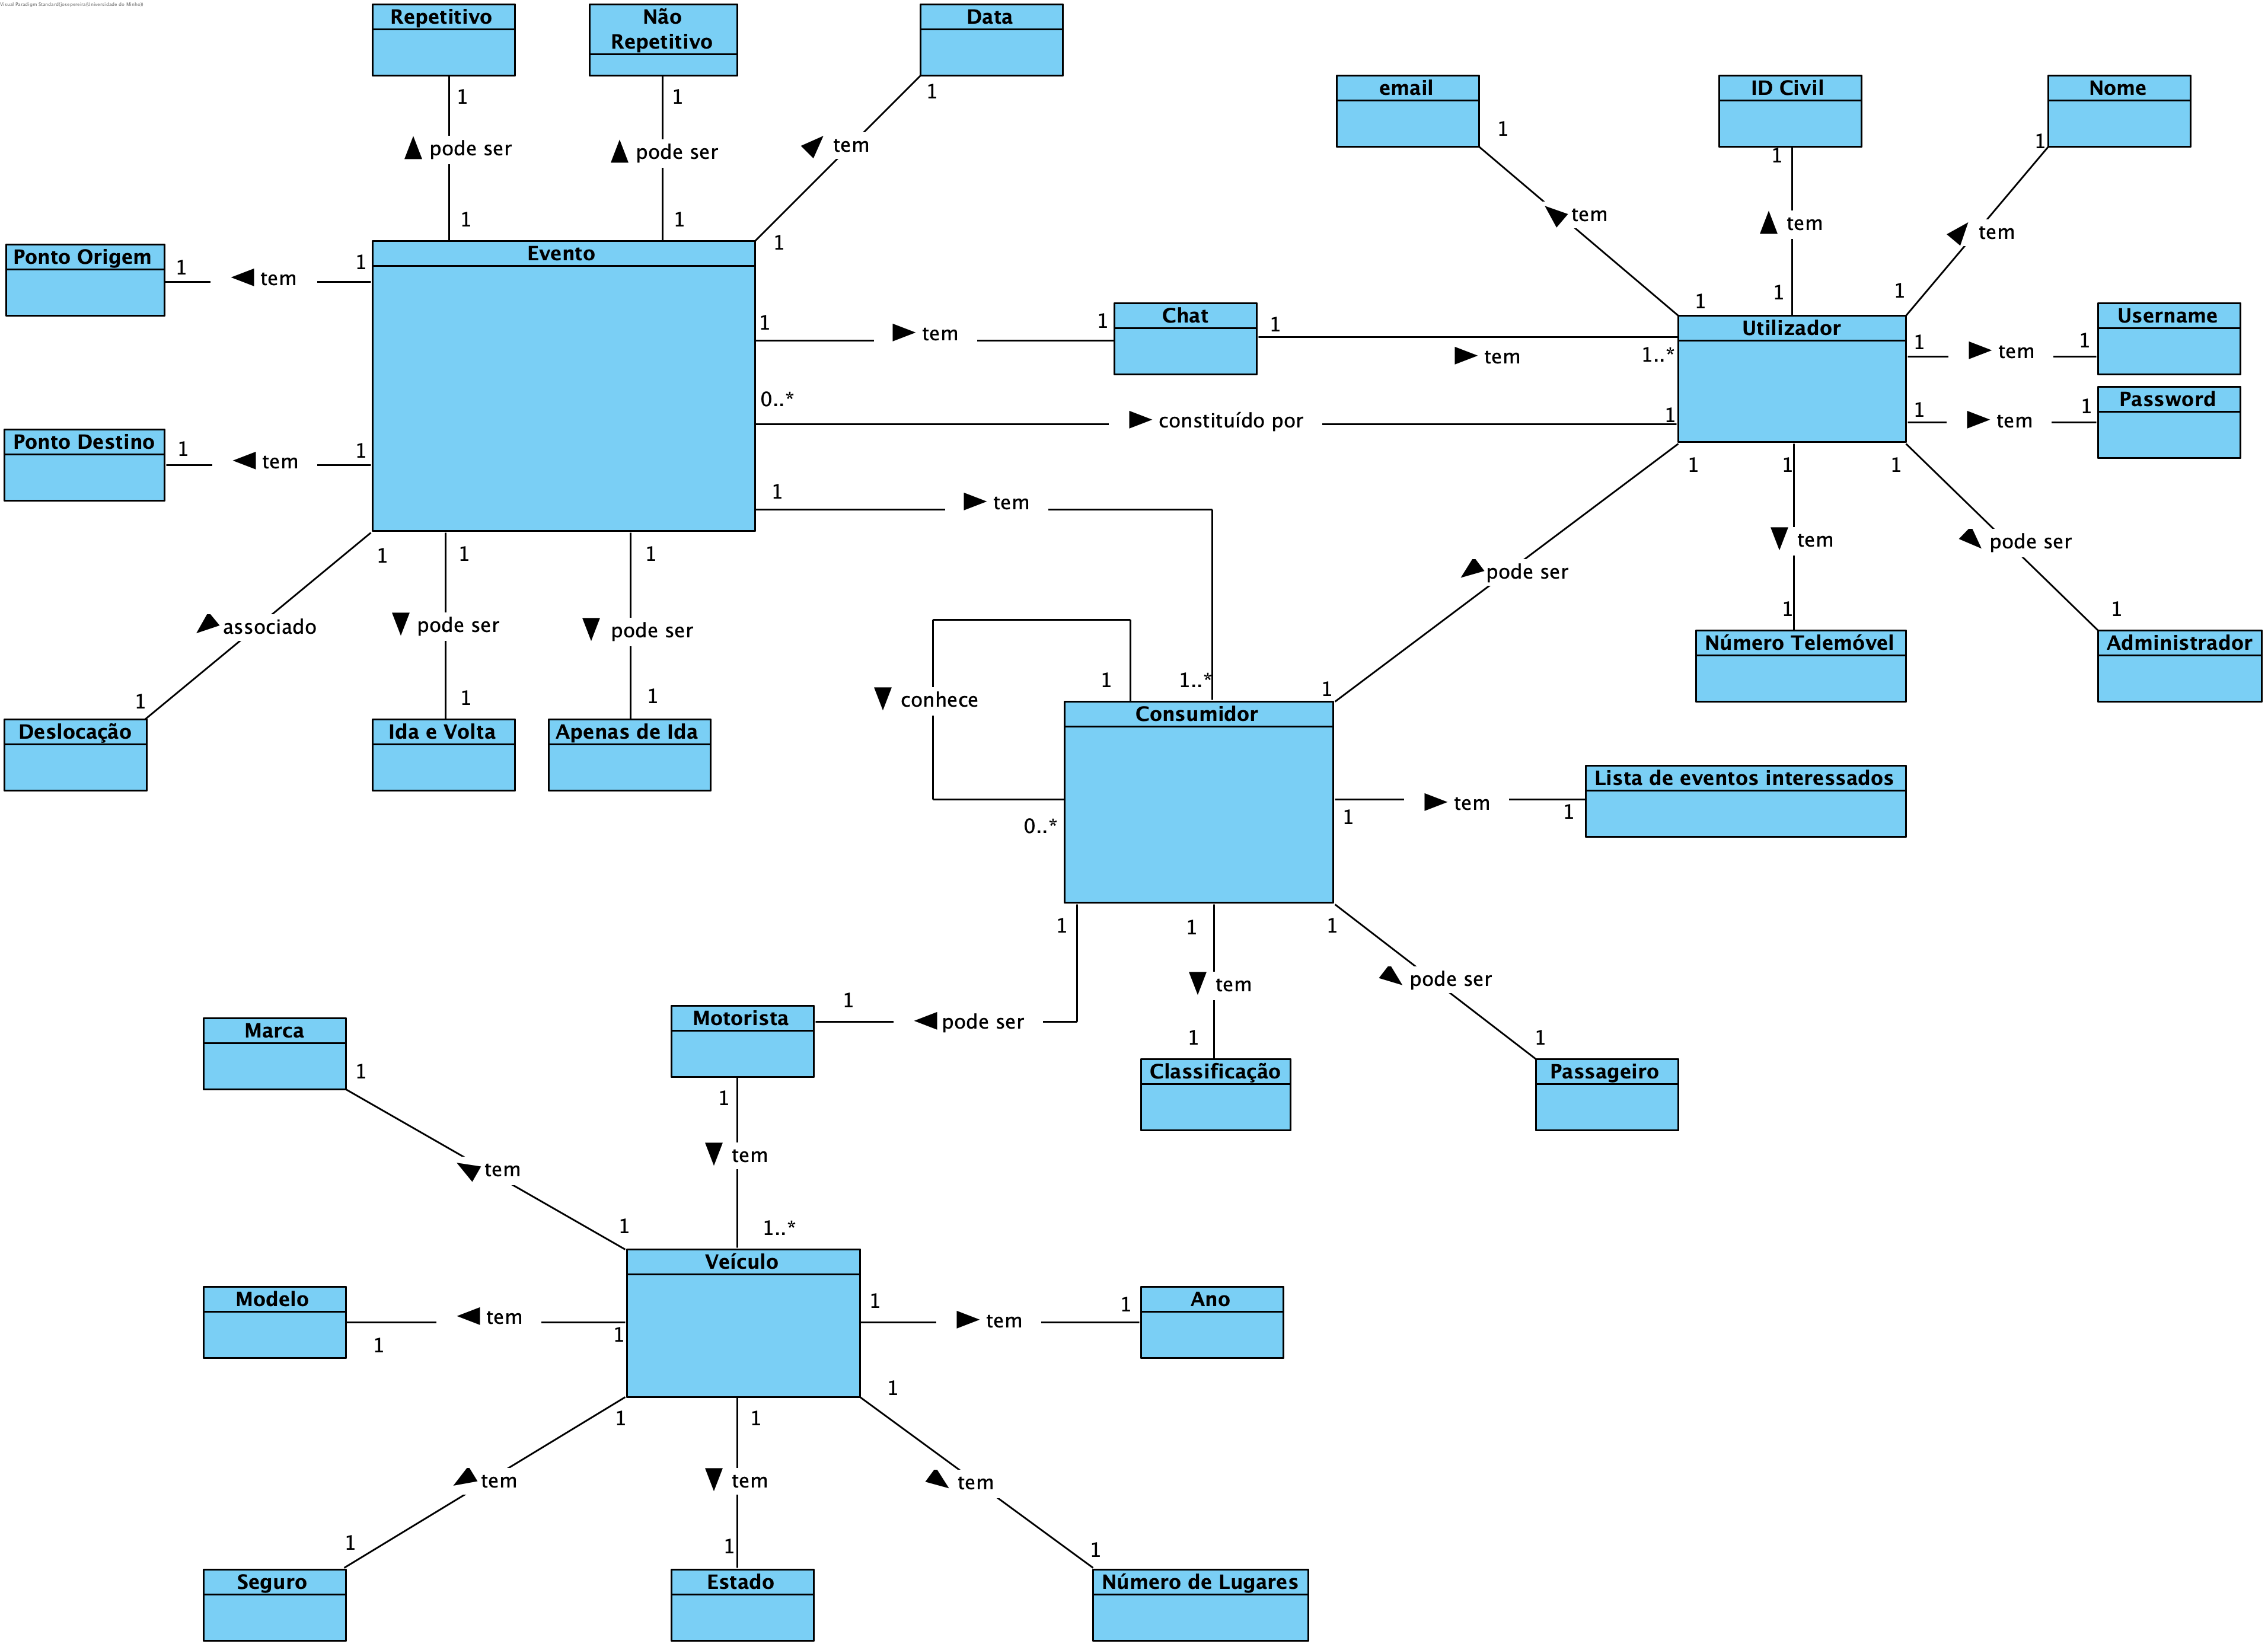
\includegraphics[scale=0.50]{modelo-dominio.png}
	\caption{Modelo Domínio.}
	\label{img:pag}
\end{figure}


\chapter{Convenções de nomenclatura e definições}

\section{Convenções de nomenclatura}
\begin{itemize}
    \item Deslocação
    \item Utilizador
    \item Viajante
    \item Administrador
    \item Perfil
    \item Classificação
    \item Comentários
    \item Veículo
    \item Chat 
\end{itemize}{}

\section{Políticas de negócio}
\hspace{5mm} Na fase inicial, o objetivo principal da aplicação centra-se em reunir pessoas, com a finalidade de efetuar uma deslocação, de forma a aproveitar os recursos automóveis, reduzindo os custos de deslocação para todos os intervenientes, bem como o trânsito. 

\section{Definições}
\begin{itemize}
    \item \textbf{Deslocação:} reunião entre utilizadores previamente planeada, organizada e coordenada de forma a contemplar o maior número de pessoas em um mesmo espaço virtual para efetuarem uma deslocação, podendo esta viagem ser frequente ou não.
    \item \textbf{Utilizador:} ator que utiliza a aplicação. O utilizador pode ser o viajante ou o administrador da aplicação.
    \item \textbf{Viajante:} são os utilizadores que efetuam as deslocações, existindo dois tipos:
    \begin{itemize}
        \item motorista
        \item passageiro
    \end{itemize}
    \item \textbf{Administrador:} utilizador da aplicação que monitoriza a mesma, através de estatísticas.
    \item \textbf{Perfil:} conjunto de informações sobre um viajante da aplicação, tais como: classificação, comentários sobre o mesmo, suas deslocações, entre outras informações.
    \item \textbf{Classifição:} está presente no perfil de cada viajante, servindo para avaliar os intervenientes numa deslocação. No fim de cada deslocação, atribui-se a cada viajante,uma classificação, sobre o seu comportamento na mesma. 
    \item \textbf{Comentários:} do mesmo modo, que a classificação, também estão associados a cada utilizador comentários sobre o comportamento do mesmo na aplicação. Os comentários são feitos no fim de cada deslocação.
    \item \textbf{Veículo:} meio de transporte que um motorista possuí para efetuar as deslocações nas quais está inserido.
    \item \textbf{Chat:} forma de comunicação em tempo real dos intervenientes de uma deslocação.
\end{itemize}{} 
\chapter{Factos Relevantes e Premissas}
\hspace{5mm} Neste capítulo, aborda-se os factos relevantes que afetam a aplicação, não estando previstos nos requisitos.

\section{Factos Relevantes}

De seguida apresentam-se factos ou mesmo obrigações legais que podem de certa forma influenciar a implementação do sistema ou alterar o seu uso por parte do consumidor. 

\begin{itemize}
    \item Legalmente o veículo necessita de ter seguro válido associado.
    \item Legalmente o motorista necessita de carta de condução válida para conduzir.
    \item Legalmente o cidadão, neste caso utilizador, necessita de ter o seu cartão de cidadão válido.
    \item Existem certas localizações, nomeadamente centros históricos das cidades, que \textbf{não} permitem deslocação por meio de veículo.
\end{itemize}

\section{Premissas}

\begin{itemize}
    \item Os veículos registados pelo motorista têm pelo menos 2 acentos.
\end{itemize}



\chapter{O âmbito do Trabalho}

\hspace{5mm} Este capítulo, refere os limites do domínio do nosso sistema por isso define o ambiente em que o mesmo se encontra. Definindo o ambiente de forma mais clara é possível detalhar com mais precisão e menor ambiguidade o domínio do sistema e ter melhor noção do impacto do novo sistema no mercado atual.

\section{A Situação Atual}

\hspace{5mm} A introdução de um novo sistema \textbf{implica sempre alterações}, caso contrário nem faria sentido o desenvolvimento e implementação desse sistema, o objetivo deve ser melhorar ou criar algo novo.

\hspace{5mm} Desta forma deve ser feito um estudo da situação atual das entidades que serão remodeladas com o objetivo de verificar como deverá ser efetuada essa alteração da forma mais eficiente.

\hspace{5mm} A própria empresa que desenvolveu a aplicação terá de realizar a \textbf{manutenção do sistema}, dessa forma a primeira alteração é a introdução de uma equipa encarregue desse trabalho.

\hspace{5mm} Visto que o novo sistema exige, por questões de segurança, que os utilizadores forneçam o seu id civil, é necessário que o cliente do sistema tenha uma equipa de recursos humanos a \textbf{fiscalizar} este documento e a sua validade.

\hspace{5mm} Do mesmo modo o seguro do veículo do motorista também necessita de ser válido e por isso fiscalizado.

\hspace{5mm} Caso o sistema tenha alta adesão por parte dos seus consumidores é possível que se verifique um diminuição de trânsito e consequente diminuição de emissões de gases prejudiciais para a atmosfera, contribuindo para uma sociedade mais sustentável.

\section{O Contexto do Trabalho}

\hspace{5mm} De forma a clarificar o domínio do sistema deve ser estudado o ambiente no qual o mesmo vai ser implementado.

\hspace{5mm} Inicialmente convém identificar \textbf{sistemas semelhantes}, neste momento o mercado contém algumas aplicações que fornecem serviços semelhantes sendo as principais: \textcolor{blue}{\href{https://www.uber.com}{uber}}, \textcolor{blue}{\href{https://bolt.eu}{bolt}} e \textcolor{blue}{\href{https://www.blablacar.pt/}{blablacar}}. Assim a equipa estudou estas aplicações de forma a identificar funcionalidades que as mesmas \textbf{não têm ou podem ser melhoradas} introduzindo-as no novo sistema a desenvolver. Outra vantagem de estudar estas aplicações é o conhecimento do estado atual da futura concorrência no mercado.

\hspace{5mm} Desta forma uma funcionalidade que foi identificada que as aplicações já existentes \textbf{não fornecem} é a possibilidade dos viajantes poderem \textbf{estabelecer o preço da deslocação entre eles sem necessitarem de efetuar transações monetárias} pela própria aplicação. Visto que é uma funcionalidade possivelmente útil e única, é uma vantagem a mesma pertencer ao novo sistema. 

\hspace{5mm} Outra funcionalidade que o sistema oferece é o \textbf{cálculo automático da estimativa do valor da deslocação}, de forma a verificar a possibilidade de implementação desta funcionalidade a equipa informou-se da existência de serviços que já realizam esta operação.

\hspace{5mm} Desta forma um serviço já existente é a api \textcolor{blue}{\href{https://api.viamichelin.com}{via-michelin}} que de acordo com as informações do carro: marca, modelo, motor, ano e tipo de combustível; o ponto de origem e ponto de destino da deslocação calcula com precisão a estimativa do custo. Note-se que apenas identificamos um possível serviço a utilizar não significa que no momento de implementação da solução, seja a melhor decisão a tomar, visto que podem existir desvantagens tais como o custo de utilização da api ou dependência de serviços externos ao sistema.








\chapter{Modelo de domínio e dicionário dos dados}

\hspace{5mm} Neste capítulo apresenta-se o modelo de dóminio do sistema bem como é detalhado cada entidade do modelo de dóminio através de um dicionário. Através destes dois modelos é feito um estudo ainda mais profundo e preciso sobre o domínio do sistema, tornando facilitado o processo de deteção de contradições ou ambiguidades e consequentemente é facilitado também o futuro processo de implementação.

\newpage
\section{Modelo de domínio}

\hspace{5mm} Na seguinte figura encontra-se o modelo de domínio criado pelo grupo.

\begin{figure}[H]
    \centering
	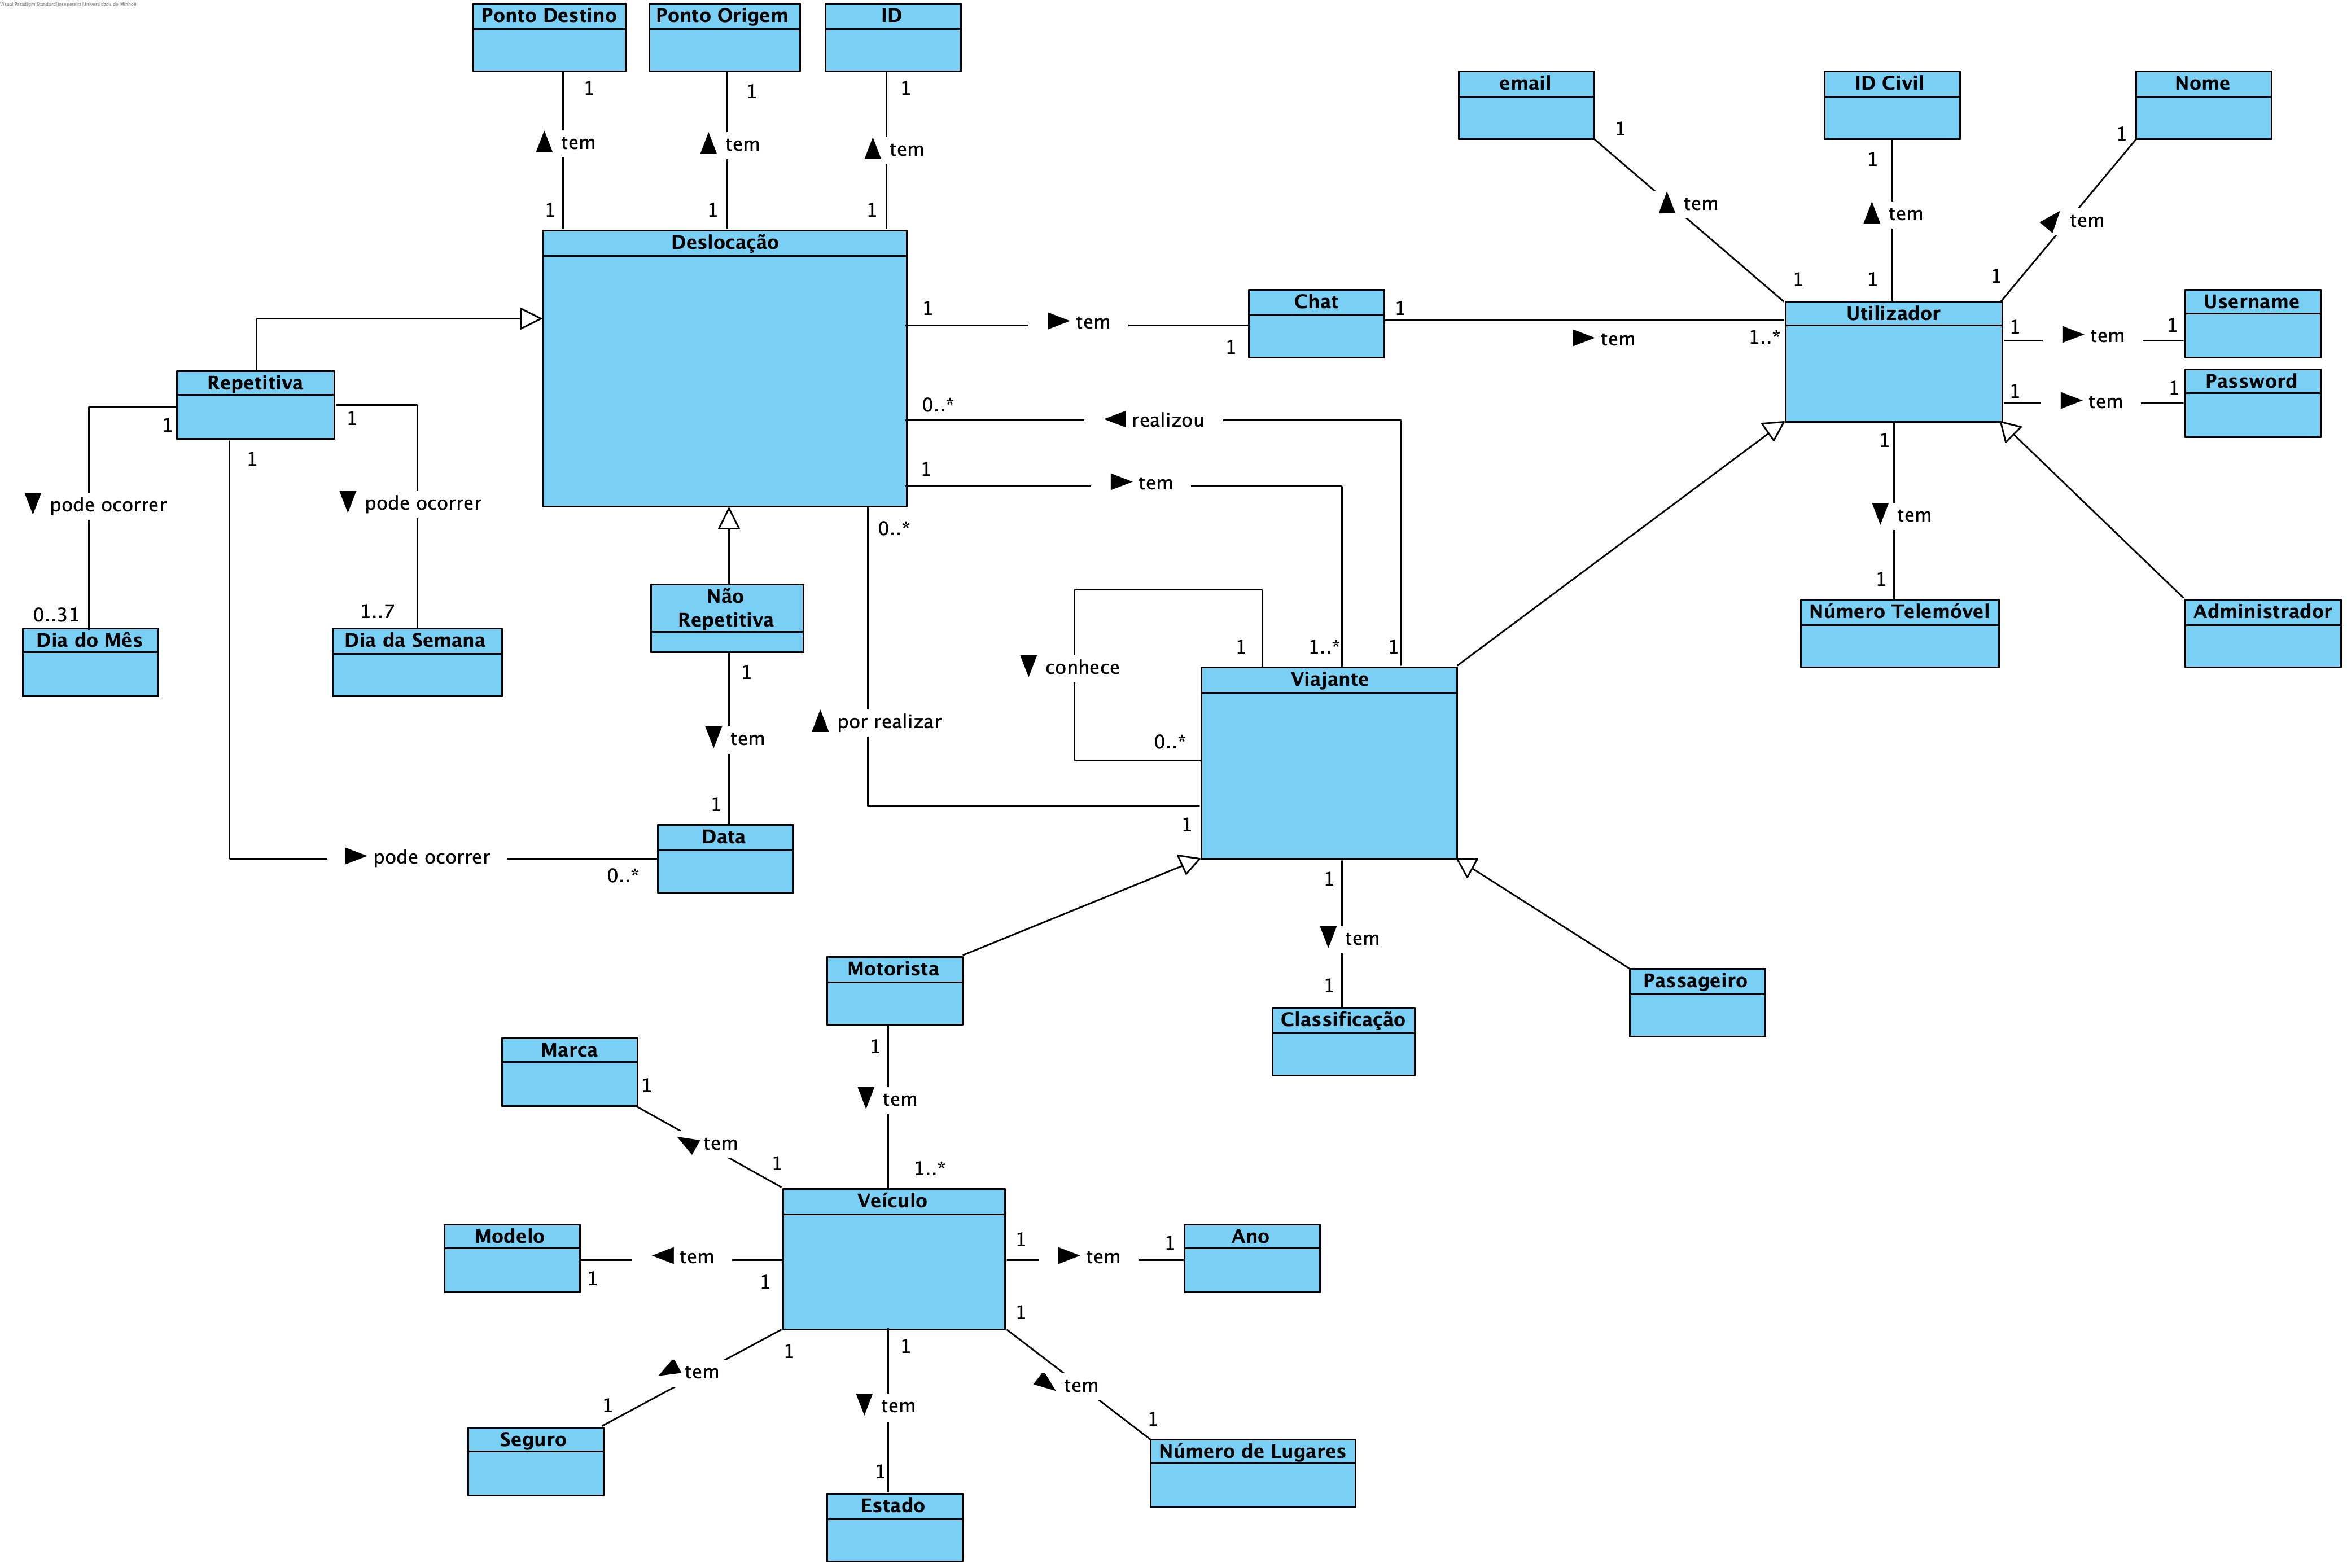
\includegraphics[scale=0.5]{imagens/modelo-dominio.png}
	\label{img:duc1}
	\caption{Modelo de dóminio do sistema.}
\end{figure}

\hspace{5mm} Inicialmente foi introduzida a noção de \textbf{utilizador} que necessita de um \textbf{username} e \textbf{password} para se autenticar no sistema, este é tratado pelo seu \textbf{nome}, pode ser contactado pelo \textbf{email} ou \textbf{número de telemóvel}, por questões de segurança também é identificado pelo seu \textbf{id civil}. 

\hspace{5mm} Desta forma existem dois tipos de utilizador: \textbf{adiministrador} ou \textbf{viajante}. Note-se que a realação entre estes dois últimos e o utilizador é de \textbf{hierarquia}, logo toda a constituição do utilizador encontra-se também no adiministrador e viajante.

\hspace{5mm} O administrador tem o papel de controlar o sistema por isso a sua \textbf{constituição não é maior} que a do utilizador, apenas as suas funcionalidades serão diferentes, isto é, poderá realizar determinadas funções de controlo que outros utilizadores não têm permissão.

\hspace{5mm} O viajante é avaliado através de uma classificação no fim de cada \textbf{deslocação}, convergindo numa única média de classificações. Este possuí um \textbf{histórico} de deslocações realizadas e também uma lista de deslocações que irá realizar. Visto que o sistema tem a funcionalidade do viajante poder seguir e ser amigo de outros viajantes, os mesmos podem \textbf{conhecer} outros. 

\hspace{5mm} Existem dois tipos de viajantes: \textbf{passageiro} e \textbf{motorista}. 

\hspace{5mm} O motorista tem pelo menos um \textbf{veículo} pertencente a uma \textbf{marca}, especificado por um \textbf{modelo}, construído num determinado \textbf{ano}, tem variável \textbf{número de lugares}, protegido com um \textbf{seguro} e necessita de estar num \textbf{estado} suficientemente seguro para se deslocar.

\hspace{5mm} Por último, provavelmente, a noção mais importante do nosso sistema é a \textbf{deslocação}. Esta é identificada internamente por um \textbf{id}, tem sempre um \textbf{ponto de origem} e \textbf{ponto de destino}, vários utilizadores podem participar num \textbf{chat} associado a uma deslocação para combinar ou clarificar algo, sendo que na mesma participam vários viajantes.

\hspace{5mm} Existem dois tipos de deslocações: \textbf{repetitivas} ou \textbf{não repetitivas}. 

\hspace{5mm} A não repetivia é um evento singular, ocorre uma única vez numa determinada \textbf{data}, por exemplo no dia 10/1/2020.

\hspace{5mm} A repetitiva pode ocorrer num \textbf{dia da semana}, por exemplo à sexta-feira, num \textbf{dia do mês}, por exemplo ao dia 20 de cada mês, ou mesmo em \textbf{datas não regulares}, por exemplo dia 20/3/2020, 18/4/2020 e 7/6/2020.  

\section{Dicionário dos dados}

\hspace{5mm} O dicionário dos dados permite estabelecer uma relação entre o domínio analisado e a futura implementação das noções abordadas. Desta forma quando o processo de implementação for realizado, os desenvolvedores têm o trabalho facilitado e entendem melhor que tipo de implementação é necessária.

\hspace{5mm} Desta forma, de seguida, apresenta-se o dicionário de dados referente ao modelo de domínio especificado anteriormente.

\begin{center}
\begin{tabular}{ | m{7em} | m{10cm}| m{4em} | } 
\hline
Nome & Constituição & tipo \\ 
\hline
Utilizador & username + password + nome + id civil + email + número de telemóvel & class \\ 
\hline
Administrador & atributos do Utilizador & class \\ 
\hline
Viajante & atributos do Utilizador + classificação + histórico de deslocações + lista de deslocações a realizar & class \\ 
\hline
Motorista & atributos do Viajante + lista de veículos & class \\
\hline
Passageiro & atributos do Viajante & class \\
\hline
Deslocação & id + ponto de origem + ponto de destino + chat + lista de viajantes & class \\
\hline
Deslocação repetitiva & atributos da Deslocação + lista de datas & class \\
\hline
Deslocação não repetitiva & atributos da Deslocação + data & class \\
\hline
username & identificador do utilizador & atributo \\
\hline
password & palavra passe de segurança do utilizador & atributo \\
\hline
nome & nome usado na comunicação com o utilizador & atributo \\
\hline
id civil & identificador civil do cartão de cidadão do utilizador & atributo \\
\hline
email & email usado na comunicação com o utilizador & atributo \\
\hline
número de telemóvel & número usado na comunicação com o utilizador & atributo \\
\hline
classificação & média de classificações do viajante & atributo \\
\hline
histórico de deslocações & lista com os identificadores de todas as deslocações já realizadas do viajante & atributo \\
\hline
lista de deslocações a realizar & lista com os identificadores de todas deslocações ainda por realizar do viajante & atributo \\
\hline
ponto de origem & localização inicial da deslocação & atributo \\
\hline
ponto de destino & localização final da deslocação & atributo \\
\hline
chat & texto utilizado para a comunicação entre utilizadores & fluxo de dados \\
\hline
lista de viajantes & lista com o username de cada viajante que participa na deslocação & atributo \\
\hline
lista de datas & lista com as datas de ínicio das deslocações & atributo \\
\hline
data & data da deslocação & atributo \\
\hline
\end{tabular}
\end{center}
\chapter{Os Limites do Produto}

\section{Limite do Produto}
\hspace{5mm} A forma utilizada para apresentar os limites do produto, consiste num diagrama de use cases, tal como podemos observar nas figuras \ref{img:duc1} \ref{img:duc2}. 

\hspace{5mm}No entanto, importanto referir, que se dividiu o diagrama de use cases em dois subsistemas, para tornar mais fácil a sua avaliação

\begin{figure}[H]
    \centering
	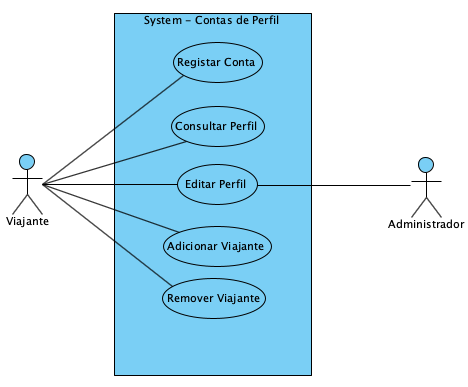
\includegraphics[scale=0.80]{imagens/diagrama-use-cases-1.png}
	\caption{Diagrama de Use cases, do subsistema relacionado com contas de utilizador.}
	\label{img:duc1}
\end{figure}

\begin{figure}[H]
    \centering
	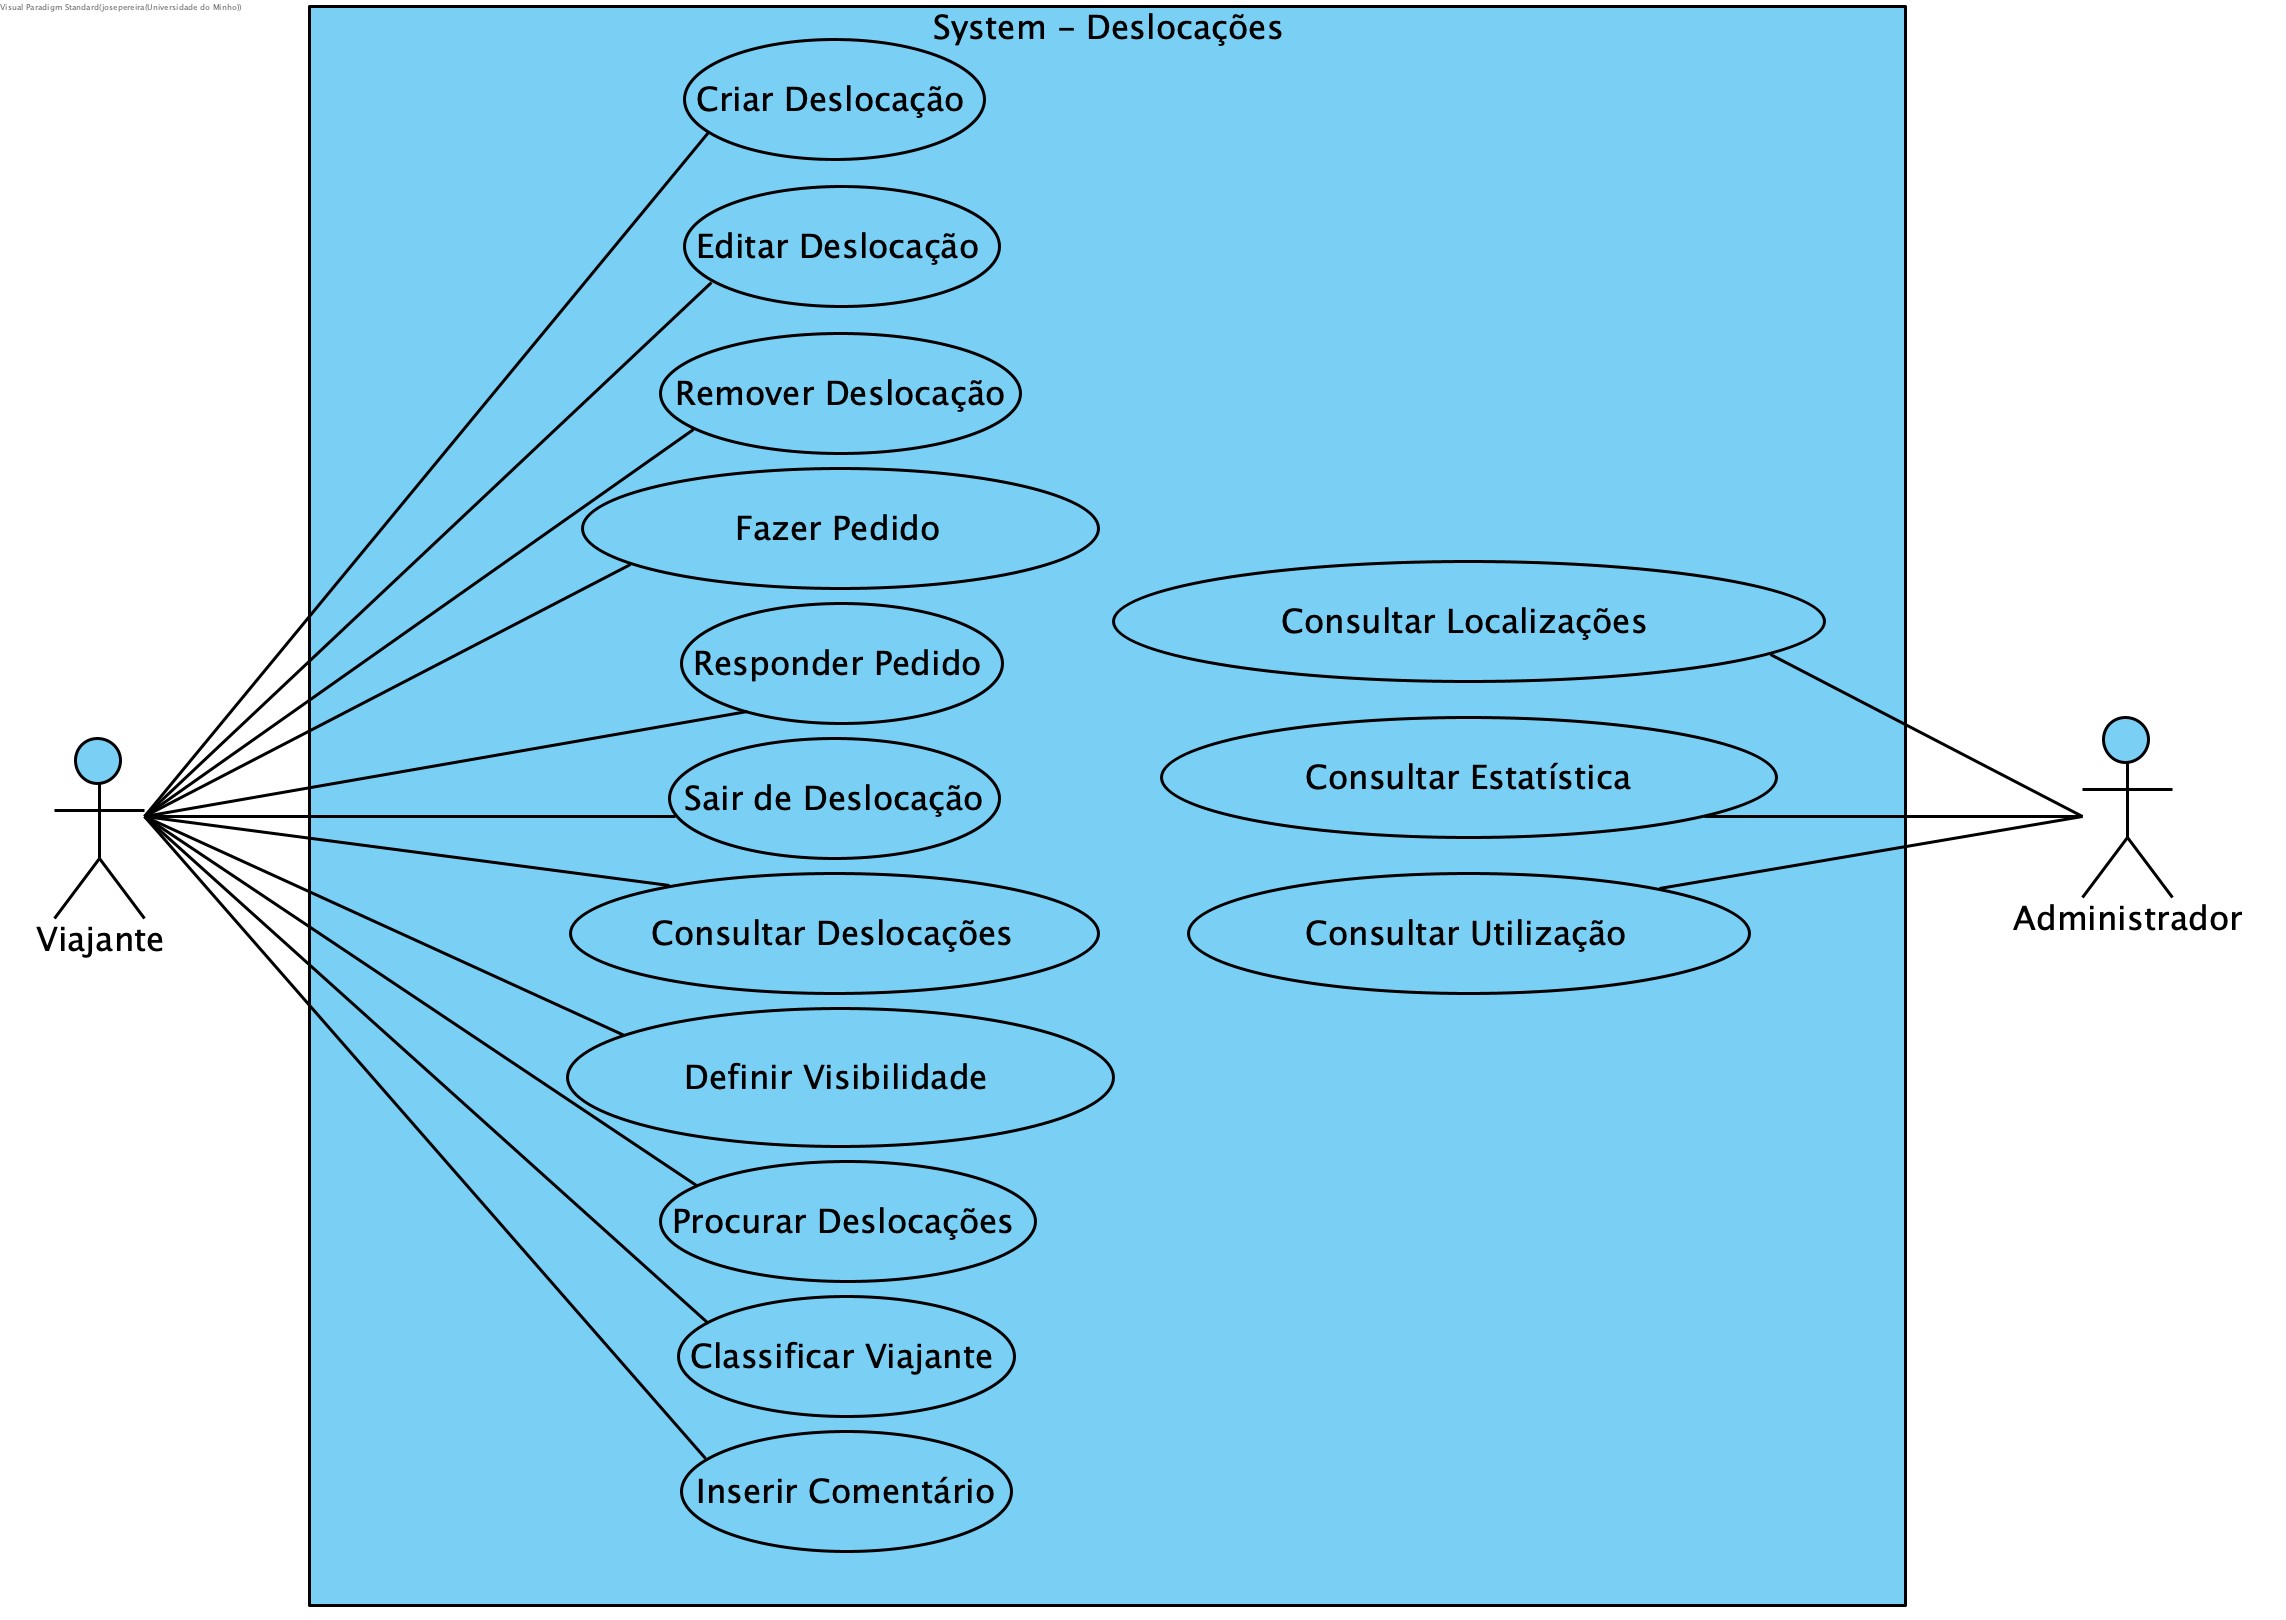
\includegraphics[scale=0.95]{imagens/diagrama-use-cases-2.png}
	\caption{Diagrama de Use cases, do subsistema relacionado com as Deslocações.}
	\label{img:duc2}
\end{figure}

\section{Tabela de \emph{Use Cases} do Produto}
\hspace{5mm} De seguida apresenta-se a tabela, com a identificação dos \emph{use cases}, os atores dos mesmos, bem como os dados de \emph{input} e \emph{output}.

\begin{table}[H]
\begin{center}
\begin{tabularx}{\textwidth}{ | c | c | c | X | }
    \hline
    Número & Nome & Atores & Input/Output \\
    
    \hline
    1 & Registar Conta & Viajante & nome, username, password, email/ mensagem de sucesso ou insucesso \\
    
    \hline
    2 & Consultar Perfil & Viajante & nome ou username/ perfil do viajante dado com input \\
    
    \hline
    3 & Editar Perfil & Viajante e Administrador & campos a serem alterados / sucesso ou insucesso da alteração \\
    
    \hline
    4 & Adicionar Viajante & Viajante & username ou nome do viajante a adicionar à lista de viajantes / sucesso ou insucesso da adição do viajante \\
    
    \hline
    5 & Remover Viajante & Viajante & username ou nome do viajante a remover da lista de viajantes / sucesso ou insucesso da remoção do viajante \\
    
    \hline
    6 & Criar Deslocação & Viajante & data, ponto origem, ponto destino, tipo (frequente, ou não frequente) / sucesso ou insucesso da criação da deslocação \\
    
    \hline
    7 & Editar Deslocação & Viajante & campos a serem alterados (não se pode alterar a origem, destino) / sucesso ou insucesso da edição da deslocação \\
    
    \hline
    8 & Remover Deslocação & Viajante & Identificador (ID) da deslocação / sucesso ou insucesso da remoção da deslocação \\
    
    \hline
    9 & Fazer Pedido & Viajante & ID da deslocação / sucesso ou insucesso da efetuação do pedido \\
    
    \hline
    10 & Responder Pedido & Viajante & aceita ou não aceita / sucesso ou insucesso da efetuação da resposta \\
    
    \hline
    11 & Sair da deslocação & Viajante & Identificador (ID) da deslocação / sucesso ou insucesso da saída da deslocação \\
    
    \hline
    12 & Consultar Deslocações & Viajante & nome ou username do viajante a consultar / lista de deslocações desse viajante \\
    
    \hline
    13 & Definir visibilidade & Viajante & tipo de visibilidade / sucesso ou insucesso da efetuação da operação \\
    
    \hline
    14 & Procurar deslocações & Viajante & filtros (origem, destino, data, tipo, etc...) / lista de deslocações encontradas \\
    
     \hline
    15 & Classificar Viajante & Viajante & valor entre zero e dez / sucesso ou insucesso da efetuação da classificação \\
    
     \hline
    16 & Inserir Comentário & Viajante & comentário / sucesso ou insucesso da inserção do comentário \\
    
     \hline
    17 & Consultar Localizações & Administrador & tipo (mais frequentes ou menos frequentes) / Lista das localizações das deslocações menos ou menos frequentes conforme o input \\
    
     \hline
    18 & Consultar Estatísticas & Administrador & tipo de estatística (métricas a avaliar) / Lista da estatística pedidas como argumento \\
    
    \hline
    19 & Consultar Utilização & Administrador & - / percentagem de utilização inteligente dos veículos total \\
    
    \hline
\end{tabularx}
\end{center}
\label{tab:r1}
\end{table}

\section{\emph{Use Case} Individualmente}

\hspace{5mm} De seguida, apresenta-se, a especificação tabular do \emph{use case} \textbf{Criar Deslocação}. Importa referir, que apenas foi feito a especificação tabular deste \emph{use case}, pois o grupo acha que se trata do mais importante.

\hspace{5mm} Importante referir que no diagrama reutilizou-se a \textbf{Exceção 1} foi usada para os vários casos de valores inválidos, visto que o processo é igual para todos, permitindo assim uma tabela mais pequena.

\newpage

\begin{figure}[H]
    \centering
	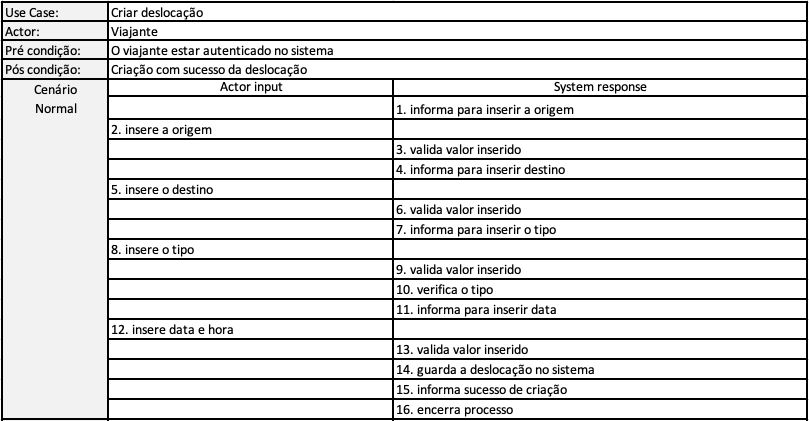
\includegraphics[scale=0.58]{imagens/use-case-especificado-1.png}
	\label{img:duc1}
\end{figure}

\begin{figure}[H]
    \centering
	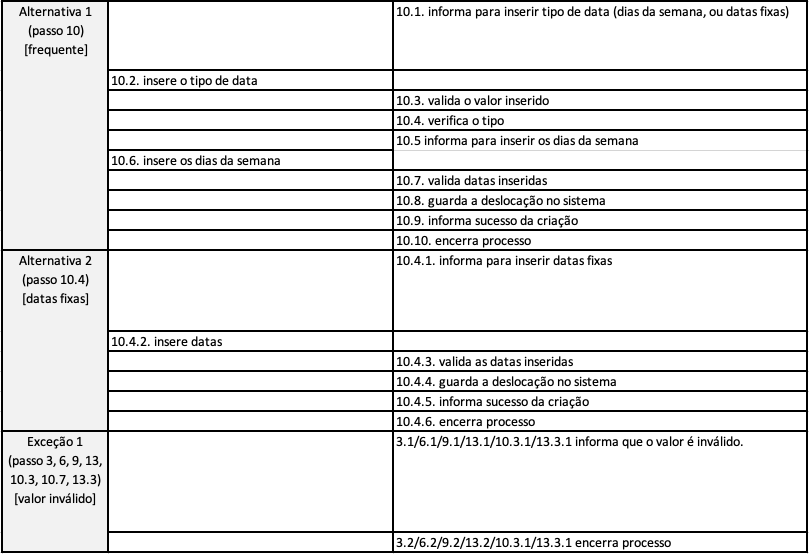
\includegraphics[scale=0.58]{imagens/use-case-especificado-2.png}
	\label{img:duc1}
	\caption{Especificação tabelar do \emph{use case} \textbf{Criar Deslocação}.}
\end{figure}
\chapter{Requisitos Funcionais}

\section{Requisitos do Utilizador}

\begin{table}[H]
\begin{center}
  \begin{tabularx}{\textwidth}{ | c | X | }
    \hline 
    Id do Requisito & 1 \\

    \hline
    Tipo de Requisito & Funcional \\
    
    \hline
    Evento, BUC, PUC & Registar Conta \\
    
    \hline
    Descrição & O viajante regista-se na aplicação. \\
    
    \hline
    Justificação do Requisito &  O viajante necessita de se identificar na aplicação para utilizar as funcionalidades da mesma e se distinguir de outros viajantes. \\
    \hline
    Origem do Requisito & Administração da empresa X. \\
    
    \hline
    Critério de Ajuste & A aplicação terá um formulário com os campos necessários para o registo do viajante, sendo os dados guardados numa base de dados.\\
    
    \hline
  \end{tabularx}
  \caption{Requisito 1.} \label{tab:r1}
\end{center}
\end{table}

\begin{table}[H]
\begin{center}
  \begin{tabularx}{\textwidth}{ | c | X | }
    \hline
    Id do Requisito & 2  \\
    
    \hline
    Tipo de Requisito & Funcional \\
    
    \hline
    Evento, BUC, PUC &  Editar Perfil\\
    
    \hline
    Descrição & O Utilizador edita o seu perfi. \\
    
    \hline
    Justificação do Requisito & O Utilizador pode necessitar de modificar as suas informações do perfil.  \\
    
    \hline
    Origem do Requisito & Administração da empresa X \\
    
    \hline
    Critério de Ajuste & O menu principal da aplicação terá a opção de editar o perfil do próprio utilizador, e as alterações efetuadas serão guardadas na base de dados.\\
    
    \hline
  \end{tabularx}
  \caption{Requisito 2.} \label{tab:r3}
\end{center}
\end{table}

\begin{table}[H]
\begin{center}
  \begin{tabularx}{\textwidth}{ | c | X | }
    \hline
    Id do Requisito & 3  \\
    
    \hline
    Tipo de Requisito & Funcional \\
    
    \hline
    Evento, BUC, PUC &  Consultar perfil\\
    
    \hline
    Descrição & O viajante consulta perfis de viajantes. \\
    
    \hline
    Justificação do Requisito & O viajante necessita de consultar o prórpio perfil, bem como o perfil de outros viajantes. \\
    
    \hline
    Origem do Requisito & Administração da empresa X \\
    
    \hline
    Critério de Ajuste & No menu principal, existe uma opção para se escrever o nome ou \emph{username}, para se procurar o perfil desse viajante, ou na lista de viajantes. \\
    
    \hline
  \end{tabularx}
  \caption{Requisito 3.} \label{tab:r3}
\end{center}
\end{table}


\begin{table}[H]
\begin{center}
  \begin{tabularx}{\textwidth}{ | c | X | }
    \hline
    Id do Requisito & 4  \\
    
    \hline
    Tipo de Requisito & Funcional \\
    
    \hline
    Evento, BUC, PUC &  Adicionar Viajante à lista\\
    
    \hline
    Descrição & O viajante adiciona à sua lista de viajantes, outros viajantes. \\
    
    \hline
    Justificação do Requisito & Alguns viajantes necessitam de guardar outros viajantes que conhecem, para poderem procurar ou partilhar as suas deslocações com os mesmos.  \\
    
    \hline
    Origem do Requisito & Administração da empresa X \\
    
    \hline
    Critério de Ajuste & No menu principal, existirá uma opção onde se poderá consultar a lista de viajantes. Desta forma, também existirá a opção de adicionar mais viajantes a essa lista, que por suas vez é guardada na base de dados.\\
    
    \hline
  \end{tabularx}
  \caption{Requisito 4.} \label{tab:r3}
\end{center}
\end{table}

\begin{table}[H]
\begin{center}
  \begin{tabularx}{\textwidth}{ | c | X | }
    \hline
    Id do Requisito & 5  \\
    
    \hline
    Tipo de Requisito & Funcional \\
    
    \hline
    Evento, BUC, PUC &  Remover Viajante da lista\\
    
    \hline
    Descrição & O viajante remove viajantes, da sua lista viajantes. \\
    
    \hline
    Justificação do Requisito & Alguns viajantes necessitam de remover outros viajantes da sua lista de viajantes por diversos motivos.  \\
    
    \hline
    Origem do Requisito & Administração da empresa X \\
    
    \hline
    Critério de Ajuste & No menu principal, existirá uma opção onde se poderá consultar a lista de viajantes. Desta forma, também existirá a opção de remover viajantes dessa lista, que por suas vez, a mesma é atualiazada na base de dados.\\
    
    \hline
  \end{tabularx}
  \caption{Requisito 5.} \label{tab:r3}
\end{center}
\end{table}


\begin{table}[H]
\begin{center}
  \begin{tabularx}{\textwidth}{ | c | X | }
    \hline
    Id do Requisito & 6  \\
    
    \hline
    Tipo de Requisito & Funcional \\
    
    \hline
    Evento, BUC, PUC &  Criar uma deslocação\\
    
    \hline
    Descrição & O viajante cria uma deslocação regular ou uma deslocação não regular. \\
    
    \hline
    Justificação do Requisito & Sendo as deslocações, o objetivo principal, faz sentido que sejam os viajantes a criá-las, podendo ser estas regulares, ou seja, que se realizam periódicamente em determinadas datas, e não regulares, ou seja, que ocorrem uma única vez.  \\
    
    \hline
    Origem do Requisito & Administração da empresa X \\
    
    \hline
    Critério de Ajuste & No menu principal existirá uma opção para criar deslocações, após se carregar na mesma, aparece um formulário, para preencher os vários campos necessários, tais como ser regular ou não regular, datas, etc.\\
    
    \hline
  \end{tabularx}
  \caption{Requisito 6.} \label{tab:r3}
\end{center}
\end{table}



\begin{table}[H]
\begin{center}
  \begin{tabularx}{\textwidth}{ | c | X | }
    \hline
    Id do Requisito & 7  \\
    
    \hline
    Tipo de Requisito & Funcional \\
    
    \hline
    Evento, BUC, PUC &  Consultar Deslocações\\
    
    \hline
    Descrição & O viajante consulta listas de deslocações. \\
    
    \hline
    Justificação do Requisito & Sendo as deslocações, o objetivo principal, faz sentido, que os viajantes possam consultar as suas deslocações e de outros viajantes.  \\
    
    \hline
    Origem do Requisito & Administração da empresa X \\
    
    \hline
    Critério de Ajuste & No menu principal, existe uma opção para consultar a lista de deslocações, sendo estas as criadas pelo próprio viajante, ou nas que este vai partipar. Um viajante pode consultar a lista de deslocações de outro viajante no seu perfil.\\
    
    \hline
  \end{tabularx}
  \caption{Requisito 7.} \label{tab:r3}
\end{center}
\end{table}

\begin{table}[H]
\begin{center}
  \begin{tabularx}{\textwidth}{ | c | X | }
    \hline
    Id do Requisito & 8  \\
    
    \hline
    Tipo de Requisito & Funcional \\
    
    \hline
    Evento, BUC, PUC &  Remover Deslocação\\
    
    \hline
    Descrição & O viajante remove uma deslocação criada pelo próprio. \\
    
    \hline
    Justificação do Requisito & Na ocorrência da impossibilidade de efetuar a deslocação, atempadamente o criador da deslocação, pode remover a mesma.  \\
    
    \hline
    Origem do Requisito & Administração da empresa X \\
    
    \hline
    Critério de Ajuste & No menu principal, existe uma opção para consultar a lista de deslocações, após esta consulta, selecionando uma deslocação, existe a opção de remover essa deslocação. No entanto, o viajante só poderá remover deslocações que tenham sido criadas pelo próprio.\\
    
    \hline
  \end{tabularx}
  \caption{Requisito 8.} \label{tab:r3}
\end{center}
\end{table}

\begin{table}[H]
\begin{center}
  \begin{tabularx}{\textwidth}{ | c | X | }
    \hline
    Id do Requisito & 9  \\
    
    \hline
    Tipo de Requisito & Funcional \\
    
    \hline
    Evento, BUC, PUC &  Editar Deslocação\\
    
    \hline
    Descrição & O viajante edita uma deslocação criada pelo próprio. \\
    
    \hline
    Justificação do Requisito & O criador da deslocação pode modificar as informações associadas à mesma, tais como: data e hora de ínicio, etc.\\
    
    \hline
    Origem do Requisito & Administração da empresa X \\
    
    \hline
    Critério de Ajuste & No menu principal, existe uma opção para consultar a lista de deslocações. Nessa lista, o viajante, seleciona-se uma deslocação que tenha sido criada pelo próprio, e existirá a opção de editar essa deslocação, onde ocorrerá um formulário, com os campos que podem ser alterados. Importante referir, que só será possível editar deslocações até dois dias antes da sua realização.\\
    
    \hline
  \end{tabularx}
  \caption{Requisito 9.} \label{tab:r3}
\end{center}
\end{table}

\begin{table}[H]
\begin{center}
  \begin{tabularx}{\textwidth}{ | c | X | }
    \hline
    Id do Requisito & 10  \\
    
    \hline
    Tipo de Requisito & Funcional \\
    
    \hline
    Evento, BUC, PUC &  Fazer Pedido\\
    
    \hline
    Descrição & O viajante faz um pedido para entrar numa deslocação de outro viajante. \\
    
    \hline
    Justificação do Requisito & O viajante necessita de fazer pedido para entrar nas deslocações de outros viajantes. No entanto, após efetuar o pedido, o viajante, fica à espera da resposta, do criador da deslocação. \\
    
    \hline
    Origem do Requisito & Administração da empresa X \\
    
    \hline
    Critério de Ajuste & Quando o viajante consulta as deslocações de outros viajantes, ao selecionar uma dessas deslocações, tem a opção de fazer pedido para entrar nas mesmas. \\
    
    \hline
  \end{tabularx}
  \caption{Requisito 10.} \label{tab:r3}
\end{center}
\end{table}


\begin{table}[H]
\begin{center}
  \begin{tabularx}{\textwidth}{ | c | X | }
    \hline
    Id do Requisito & 11  \\
    
    \hline
    Tipo de Requisito & Funcional \\
    
    \hline
    Evento, BUC, PUC &  Responder a Pedido\\
    
    \hline
    Descrição & O viajante, nas deslocações criadas por ele, aceita ou não aceita o pedido de outro viajante para entrar nessa deslocação. \\
    
    \hline
    Justificação do Requisito & Visto que são feitos pedidos para se entrar em deslocações, necessita-se de uma aprovação das mesmas. Deste modo, decidiu-se que o criador das deslocações, aceita ou rejeita esses pedidos.  \\
    
    \hline
    Origem do Requisito & Administração da empresa X \\
    
    \hline
    Critério de Ajuste & Quando o viajante consulta as deslocações de outros viajantes, ao selecionar uma dessas deslocações, tem a opção de fazer pedido para entrar nas mesmas. \\
    
    \hline
  \end{tabularx}
  \caption{Requisito 11.} \label{tab:r3}
\end{center}
\end{table}

\begin{table}[H]
\begin{center}
  \begin{tabularx}{\textwidth}{ | c | X | }
    \hline
    Id do Requisito & 12  \\
    
    \hline
    Tipo de Requisito & Funcional \\
    
    \hline
    Evento, BUC, PUC &  Definir Visibilidade\\
    
    \hline
    Descrição & O viajante define a visibilidade da sua lista de deslocações para restantes viajantes. \\
    
    \hline
    Justificação do Requisito & Através dos inquéritos e entrevistas, precebeu-se que os viajantes presam pela sua privacidade. Deste modo, os mesmo decidem, quem poderá ver as suas deslocações.  \\
    
    \hline
    Origem do Requisito & Inquéritos realizados aos alunos da Universidade do Minho \\
    
    \hline
    Critério de Ajuste & O Viajante ao consultar a sua lista de deslocações, existe a opção de visibilidade, onde se poderá definir, quem pode consultr essa mesma lista.  \\
    
    \hline
  \end{tabularx}
  \caption{Requisito 12.} \label{tab:r3}
\end{center}
\end{table}

\begin{table}[H]
\begin{center}
  \begin{tabularx}{\textwidth}{ | c | X | }
    \hline
    Id do Requisito & 13  \\
    
    \hline
    Tipo de Requisito & Funcional \\
    
    \hline
    Evento, BUC, PUC &  Classificar Viajante\\
    
    \hline
    Descrição & O viajante, no fim de uma deslocação, atribuí uma classificação a todos os viajantes participantes dessa deslocação. \\
    
    \hline
    Justificação do Requisito & Analisando aplicações idênticas a estas, verfica-se a existência de uma forma de avaliação da atitude dos utilizadores nas aplicações. Do mesmo, nas entrevistas realizadas, também foi sempre uma sugestão recorrente a utilização da classificação para essas avaliações.  \\
    
    \hline
    Origem do Requisito & Entrevistas e Inquéritos realizados aos alunos da Universidade do Minho \\
    
    \hline
    Critério de Ajuste & Quando o criador assinalar a finalização da deslocação ou chegar-se à hora marcada como fim da deslocação, o criador e todos os intrevenientes dessa mesma deslocação, vão receber na aplicação uma questionário, para classificar o comportamento de cada viajante.  \\
    
    \hline
  \end{tabularx}
  \caption{Requisito 13.} \label{tab:r3}
\end{center}
\end{table}

\begin{table}[H]
\begin{center}
  \begin{tabularx}{\textwidth}{ | c | X | }
    \hline
    Id do Requisito & 14  \\
    
    \hline
    Tipo de Requisito & Funcional \\
    
    \hline
    Evento, BUC, PUC &  Inserir Comentário\\
    
    \hline
    Descrição & O viajante, no fim de uma deslocação, atribuí comentários a todos os viajantes participantes dessa deslocação.\\
    
    \hline
    Justificação do Requisito & Analisando aplicações idênticas a estas, verfica-se a existência de uma forma de avaliação da atitude dos utilizadores nas aplicações. Do mesmo, nas entrevistas realizadas, também foi sempre uma sugestão recorrente a utilização de comentários para essas avaliações.  \\
    
    \hline
    Origem do Requisito & Entrevistas e Inquéritos realizados aos alunos da Universidade do Minho \\
    
    \hline
    Critério de Ajuste & Quando o criador assinalar a finalização da deslocação ou chegar-se à hora marcada como fim da deslocação, o criador e todos os intrevenientes dessa mesma deslocação, irão ter trinta minutos, para poderem adicionar comentários sobre o comportamento de cada viajante.  \\
    
    \hline
  \end{tabularx}
  \caption{Requisito 14.} \label{tab:r3}
\end{center}
\end{table}

\begin{table}[H]
\begin{center}
  \begin{tabularx}{\textwidth}{ | c | X | }
    \hline
    Id do Requisito & 15  \\
    
    \hline
    Tipo de Requisito & Funcional \\
    
    \hline
    Evento, BUC, PUC &  Procurar Deslocações\\
    
    \hline
    Descrição & O viajante procura deslocações.\\
    
    \hline
    Justificação do Requisito & Como o principal objetivo da aplicação é efetuar deslocações, é necessário fazer a procura das mesmas. \\
    
    \hline
    Origem do Requisito & Addministração da empresa X\\
    
    \hline
    Critério de Ajuste & No menu principal existe uma opção de procura por deslocações, onde se pode usar filtros (como por exemplo: origem, destino, datas, tipo de veículo, etc...), para facilitar essa procura.  \\
    
    \hline
  \end{tabularx}
  \caption{Requisito 15.} \label{tab:r3}
\end{center}
\end{table}

\begin{table}[H]
\begin{center}
  \begin{tabularx}{\textwidth}{ | c | X | }
    \hline
    Id do Requisito & 16  \\
    
    \hline
    Tipo de Requisito & Funcional \\
    
    \hline
    Evento, BUC, PUC &  Sair de Deslocação\\
    
    \hline
    Descrição & O viajante sair de uma deslocação.\\
    
    \hline
    Justificação do Requisito & Do mesmo modo, que se permite que os viajantes entrem em deslocações, também necessita-se de permitir que os mesmos possam sair. \\
    
    \hline
    Origem do Requisito & Entrevista com stackholders\\
    
    \hline
    Critério de Ajuste & O viajante, ao consultar as deslocações em que vai participar, pode selecionar, uma dessas deslocações, para deixar de participar na mesma, existe a opção de sair.  \\
    
    \hline
  \end{tabularx}
  \caption{Requisito 16.} \label{tab:r3}
\end{center}
\end{table}

\begin{table}[H]
\begin{center}
  \begin{tabularx}{\textwidth}{ | c | X | }
    \hline
    Id do Requisito & 17  \\
    
    \hline
    Tipo de Requisito & Funcional \\
    
    \hline
    Evento, BUC, PUC &  Consultar Estatística\\
    
    \hline
    Descrição & O Administrador consulta número de Utilizadores.\\
    
    \hline
    Justificação do Requisito & Entrevistas realizadas à administração da empresa X, percebeu-se a importância do número de utilizadores a aderir a projetos, para contribuição do meio ambiente. \\
    
    \hline
    Origem do Requisito & Adminitração da empresa X\\
    
    \hline
    Critério de Ajuste & No menu de administrador existe a opção para consultar o número de utilizadores.  \\
    
    \hline
  \end{tabularx}
  \caption{Requisito 17.} \label{tab:r3}
\end{center}
\end{table}

\begin{table}[H]
\begin{center}
  \begin{tabularx}{\textwidth}{ | c | X | }
    \hline
    Id do Requisito & 17  \\
    
    \hline
    Tipo de Requisito & Funcional \\
    
    \hline
    Evento, BUC, PUC &  Consultar Estatística\\
    
    \hline
    Descrição & O Administrador consulta número de deslocações.\\
    
    \hline
    Justificação do Requisito & Entrevistas realizadas à administração da empresa X, percebeu-se a importância do número de deslocações, efetuadas, para efeitos estatísticos. \\
    
    \hline
    Origem do Requisito & Adminitração da empresa X\\
    
    \hline
    Critério de Ajuste & No menu de administrador existe a opção para consultar o número de deslocações.  \\
    
    \hline
  \end{tabularx}
  \caption{Requisito 17.} \label{tab:r3}
\end{center}
\end{table}

\begin{table}[H]
\begin{center}
  \begin{tabularx}{\textwidth}{ | c | X | }
    \hline
    Id do Requisito & 18  \\
    
    \hline
    Tipo de Requisito & Funcional \\
    
    \hline
    Evento, BUC, PUC &  Consultar localizações\\
    
    \hline
    Descrição & O Administrador consulta as localizações das deslocações, com mais ocorrências.\\
    
    \hline
    Justificação do Requisito & Entrevistas realizadas à administração da empresa X, percebeu-se a importância da localização das deslocações que mais ocorrem, para se saber onde encontrar os utilizadores, para possíveis melhorias do produto no futuro. \\
    
    \hline
    Origem do Requisito & Adminitração da empresa X\\
    
    \hline
    Critério de Ajuste & No menu de administrador existe a opção para consultar as localizações das deslocações que mais ocorrem.  \\
    
    \hline
  \end{tabularx}
  \caption{Requisito 18.} \label{tab:r3}
\end{center}
\end{table}

\begin{table}[H]
\begin{center}
  \begin{tabularx}{\textwidth}{ | c | X | }
    \hline
    Id do Requisito & 19  \\
    
    \hline
    Tipo de Requisito & Funcional \\
    
    \hline
    Evento, BUC, PUC &  Consultar localizações\\
    
    \hline
    Descrição & O Administrador consulta as localizações das deslocações, com menos ocorrências.\\
    
    \hline
    Justificação do Requisito & Entrevistas realizadas à administração da empresa X, percebeu-se a importância da localização das deslocações que menos ocorrem, para se saber onde é necessário investir em publicidade do produto, para maior aderência. \\
    
    \hline
    Origem do Requisito & Adminitração da empresa X\\
    
    \hline
    Critério de Ajuste & No menu de administrador existe a opção para consultar as localizações das deslocações que menos ocorrem.  \\
    
    \hline
  \end{tabularx}
  \caption{Requisito 19.} \label{tab:r3}
\end{center}
\end{table}


\begin{table}[H]
\begin{center}
  \begin{tabularx}{\textwidth}{ | c | X | }
    \hline
    Id do Requisito & 20  \\
    
    \hline
    Tipo de Requisito & Funcional \\
    
    \hline
    Evento, BUC, PUC &  Consultar Estatística\\
    
    \hline
    Descrição & O Administrador consulta os custos totais de todas as deslocações.\\
    
    \hline
    Justificação do Requisito & Entrevistas realizadas à administração da empresa X, percebeu-se a importância do cálculo dos custos totais das deslocações, para se ver o impacto monetário, que a aplicação teve nos utilizadores. Isto é, para efeitos estatísticos, perceber, o valor monetário, que foi poupado pelos utilizadores, versus o valor que gastariam infividualmente. \\
    
    \hline
    Origem do Requisito & Adminitração da empresa X\\
    
    \hline
    Critério de Ajuste & No menu de administrador existe a opção para consultar o valor dos custos de todas as deslocações.  \\
    
    \hline
  \end{tabularx}
  \caption{Requisito 20.} \label{tab:r3}
\end{center}
\end{table}

\begin{table}[H]
\begin{center}
  \begin{tabularx}{\textwidth}{ | c | X | }
    \hline
    Id do Requisito & 21  \\
    
    \hline
    Tipo de Requisito & Funcional \\
    
    \hline
    Evento, BUC, PUC &  Consultar Utilização\\
    
    \hline
    Descrição & O Administrador consulta a utilização dos veículos.\\
    
    \hline
    Justificação do Requisito & Entrevistas realizadas à administração da empresa X, percebeu-se a importância do cálculo da percentagem de utilização dos recursos dos veículos, isto é, o número de lugares utilizados, versus os lugares existentes. Na verdade, este cálculo, torna-se importante para se perceber o impacto do produto para a contribuição da utilização inteligente dos veículos. \\
    
    \hline
    Origem do Requisito & Adminitração da empresa X\\
    
    \hline
    Critério de Ajuste & No menu de administrador existe a opção para consultar a utilização dos veículos.  \\
    
    \hline
  \end{tabularx}
  \caption{Requisito 21.} \label{tab:r3}
\end{center}
\end{table}



\section{Requisitos de Sistema}

\begin{table}[H]
\begin{center}
  \begin{tabularx}{\textwidth}{ | c | X | }
    \hline
    Id do Requisito & 22  \\
    
    \hline
    Tipo de Requisito & Funcional \\
    
    \hline
    Evento, BUC, PUC &  - \\
    
    \hline
    Descrição & O sistema estima o custo da deslocação, antes da sua realização.\\
    
    \hline
    Justificação do Requisito & Apesar de a forma de pagamento ficar à descrição dos intrevenientes da deslocação, a aplicação cálcula e sugere um valor para o custa da mesma, com base nos quilómetros e desgastes do veículo. \\
    
    \hline
    Origem do Requisito & Entrevistas aos stackholders\\
    
    \hline
    Critério de Ajuste & Quando uma deslocação é criada, o sistema, cálcula, com base nos quilómetros e tipo de estrada, bem como o tipo de veículo, combustível, entre outras métricas, para determinar o valor aproximado do custo dessa deslocação.   \\
    
    \hline
  \end{tabularx}
  \caption{Requisito 22.} \label{tab:r3}
\end{center}
\end{table}

\begin{table}[H]
\begin{center}
  \begin{tabularx}{\textwidth}{ | c | X | }
    \hline
    Id do Requisito & 23  \\
    
    \hline
    Tipo de Requisito & Funcional \\
    
    \hline
    Evento, BUC, PUC &  - \\
    
    \hline
    Descrição & O sistema sugere deslocações ao consumidor de acordo com o histórico de uso do mesmo. \\
    
    \hline
    Justificação do Requisito & Com base em algumas entrevistas aos stackholders, recorrentemente, umas das funcionalidades essenciais, seria a recomendação de deslocações com base no histório, pois, se se pensar num exemplo, um viajante que vá regularmente de Braga para o Porto, estará sempre interessado em possíveis deslocações que façam este trajeto. \\
    
    \hline
    Origem do Requisito & Entrevistas aos stackholders\\
    
    \hline
    Critério de Ajuste & No menu principal, aparecem sugestões de deslocações com base no histórico do utilizador. Desta forma, significa, que se guarda o histórico do viajante na base de dados da aplicação.   \\
    
    \hline
  \end{tabularx}
  \caption{Requisito 23.} \label{tab:r3}
\end{center}
\end{table}

\begin{table}[H]
\begin{center}
  \begin{tabularx}{\textwidth}{ | c | X | }
    \hline
    Id do Requisito & 24  \\
    
    \hline
    Tipo de Requisito & Funcional \\
    
    \hline
    Evento, BUC, PUC &  - \\
    
    \hline
    Descrição & O sistema notifica todos os intrevenientes de uma deslocação, quando há alterações nessa mesma deslocação. \\
    
    \hline
    Justificação do Requisito & Após o criador efetuar alterações nas informações de uma deslocação, torna-se importante, informar os intrevenientes, dessas mesmas alterações. Na verdade, com essas alterações a deslocação pode já não ser viável para os restantes intrevenientes. \\
    
    \hline
    Origem do Requisito & Entrevistas aos stackholders\\
    
    \hline
    Critério de Ajuste & Quando são efetuadas alterações numa deslocação, o sistema informa todos os intrevenientes, dessa alteração, ou seja, os mesmos recebem notificação, com avisos do sucedido. \\
    
    \hline
  \end{tabularx}
  \caption{Requisito 24.} \label{tab:r3}
\end{center}
\end{table}



\chapter{Riscos associados ao Produto}
\hspace{5mm} Neste capítulo aborda-se os riscos associados à aplicação. Desta forma, existem vários riscos de segurança para os viajantes. Na verdade, nunca se sabe as pessoas que podem aparecer para a partilha do carro, pois podem ter segundas intenções, por exemplo, com o intuito de assaltar pessoas. No entanto, haverá um investimento necessário de fiscalização aos viajantes da aplicação, e obviamente a recomendação de viajarem apenas com pessoas com boa classificação ou conhecidos.

\hspace{5mm} Outros riscos possíveis relacionam-se com condução dos motoristas, que afetam todos os passageiros do veículo.

\hspace{5mm} Por outro lado, acidentes não provocados pelos motoristas, mas por questões externas, impossíveis de evitar, e que afetam todos os viajantes do veículo.

\hspace{5mm} A nível de segurança dos dados, tudo será feito para se evitar exposição dos dados indesejados, com equipas qualificadas para garantir a segurança dos mesmos, no entanto, existe sempre esse risco.

\hspace{5mm} A aplicação não consegue garantir que as pessoas vão cumprir as deslocações. No entanto, em caso de reportação dessas situações, o causador das mesmas, em caso de ausência de uma boa explicação, será desclassificado ou banido da aplicação.

\hspace{5mm}Por fim, e não menos importante, a inserção de documentação falsa (Cartão de cidadão ou seguro do carro) poderá a acontecer, no entanto, terá que existir uma equipa e mecanismos de fiscalização destes documentos.




\chapter{Anexos}
\section{Modelo Domínio}
\begin{figure}[H]
    \centering
	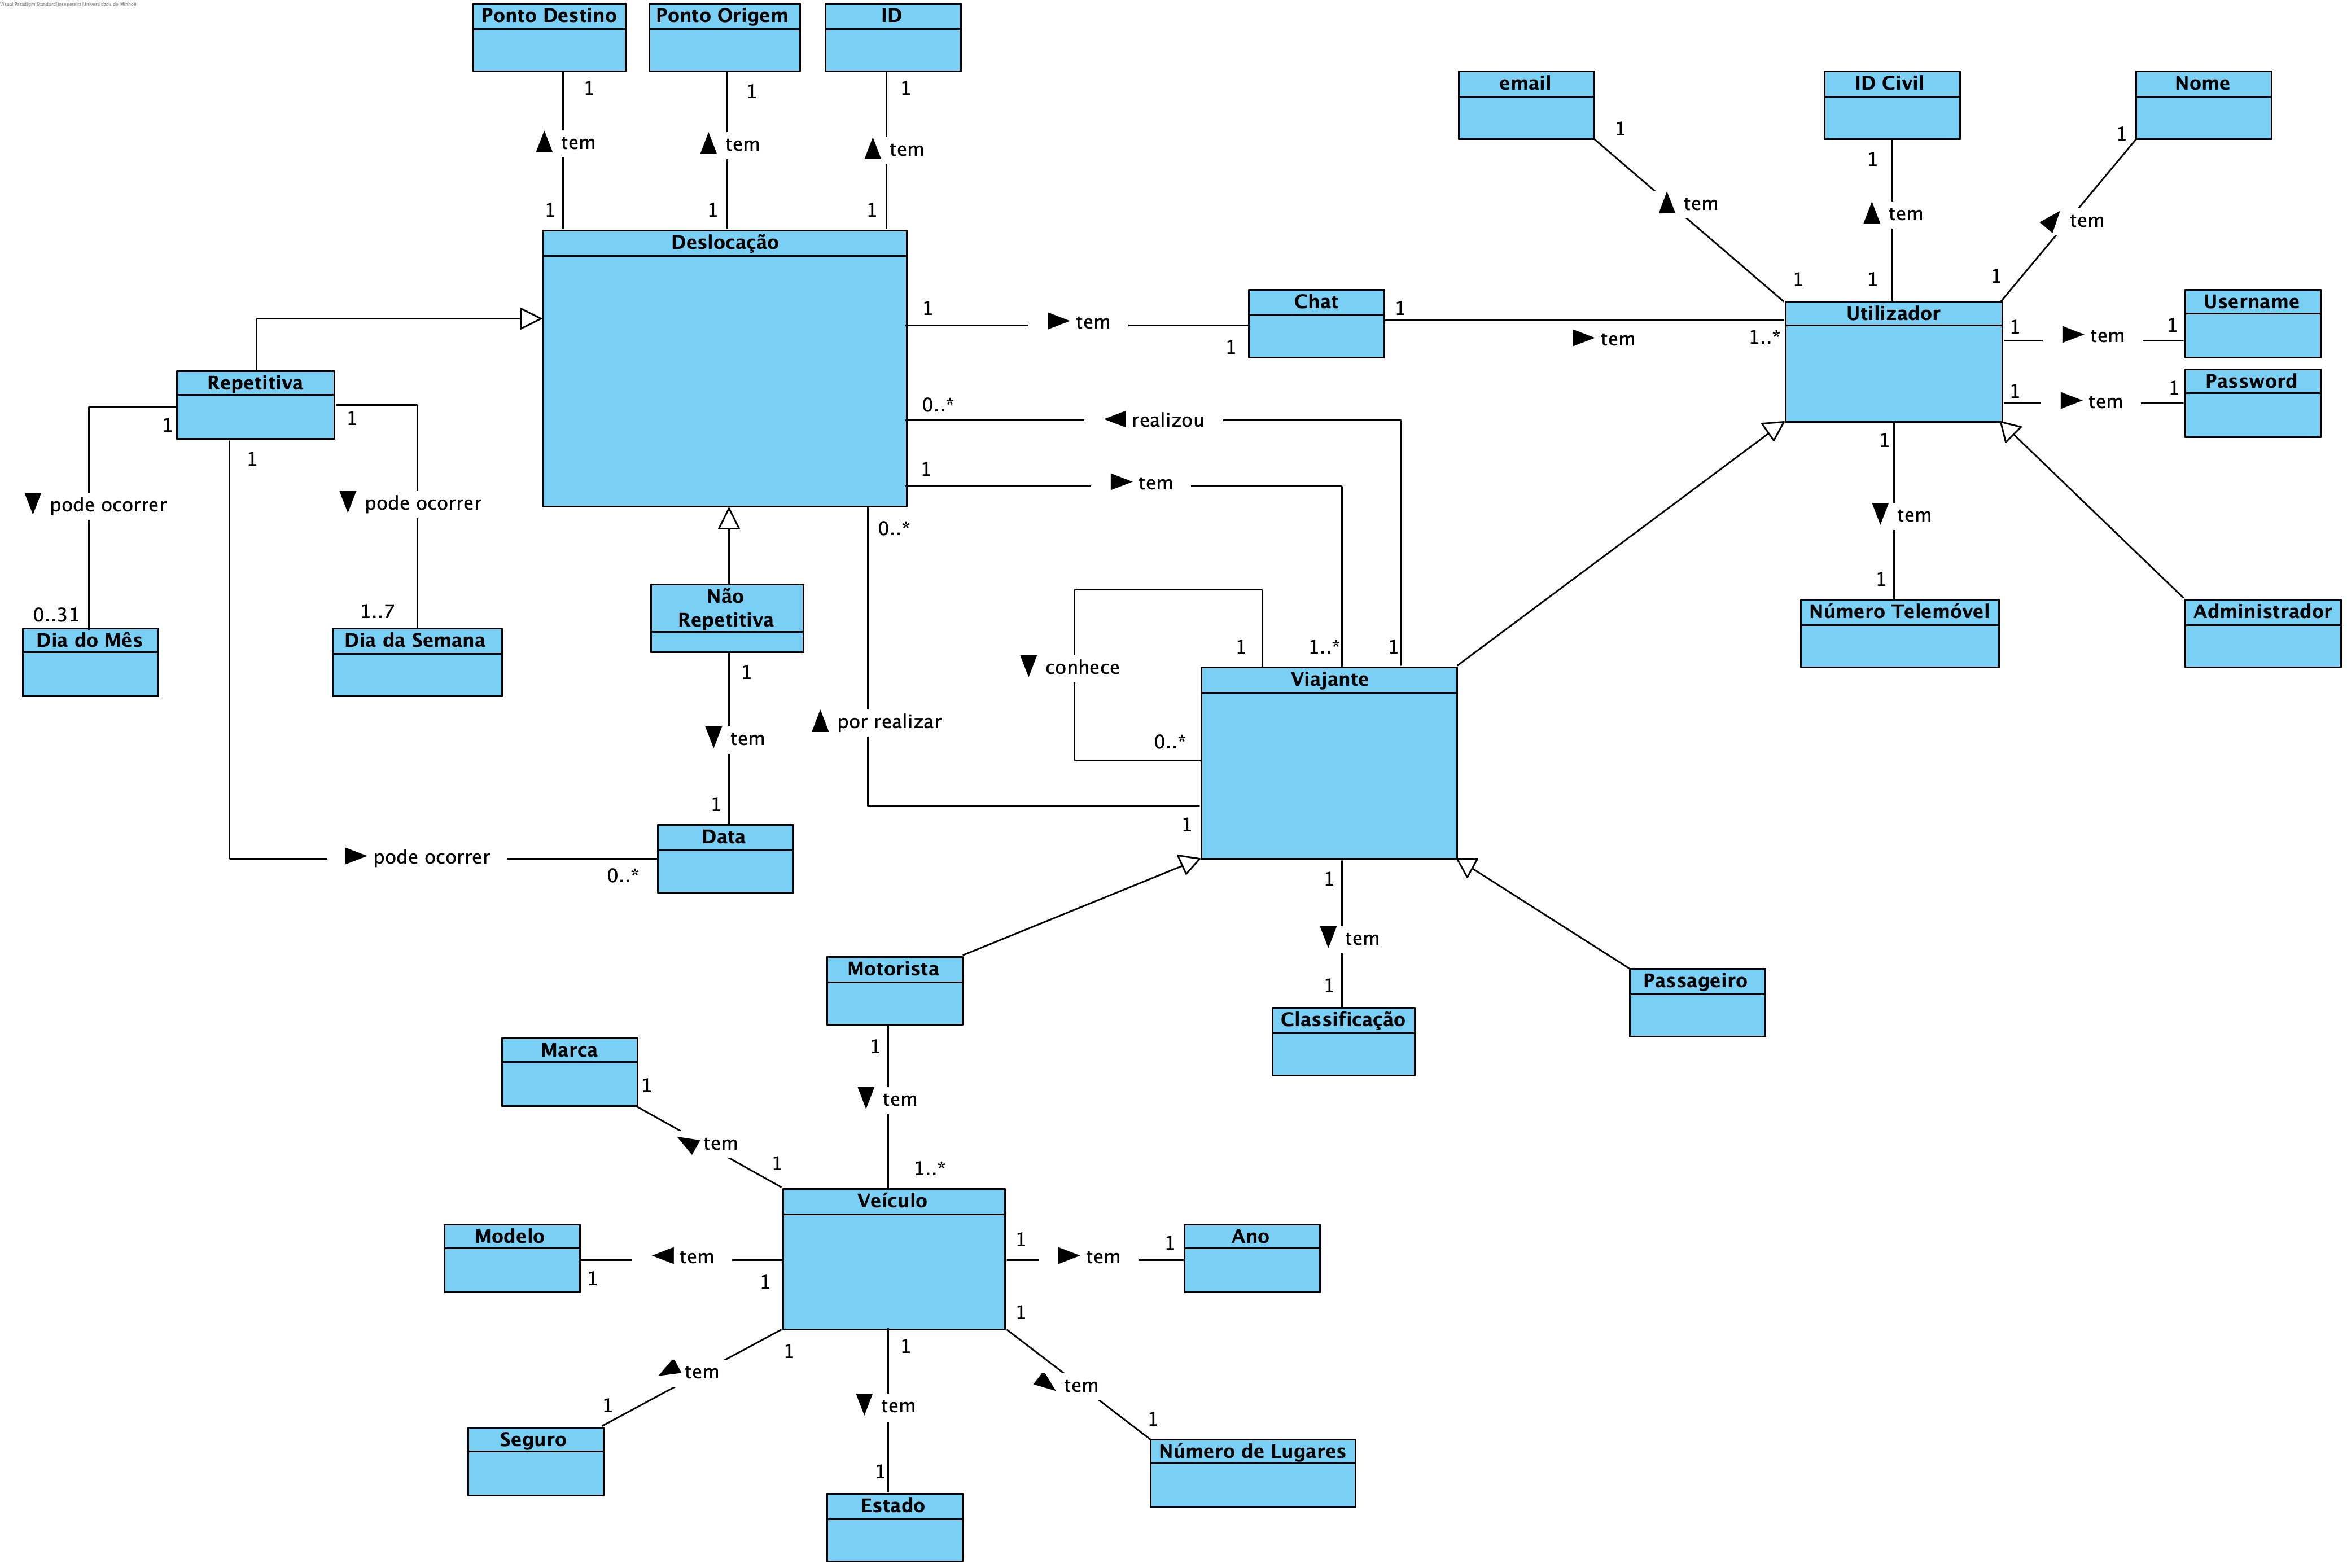
\includegraphics[scale=0.55]{imagens/modelo-dominio.png}
	\caption{Modelo Domínio.}
	\label{img:pag}
\end{figure}

\section{Diagrama de Use cases}

\begin{figure}[H]
    \centering
	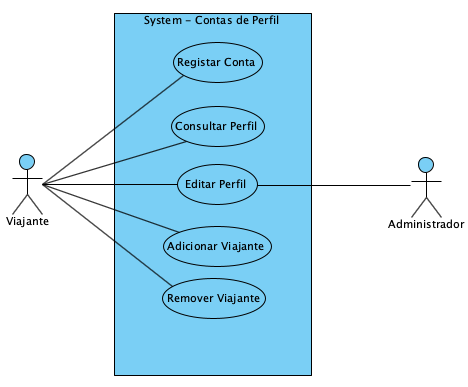
\includegraphics[scale=0.70]{imagens/diagrama-use-cases-1.png}
	\caption{Diagrama de Use cases.}
	\label{img:pag}
\end{figure}

\begin{figure}[H]
    \centering
	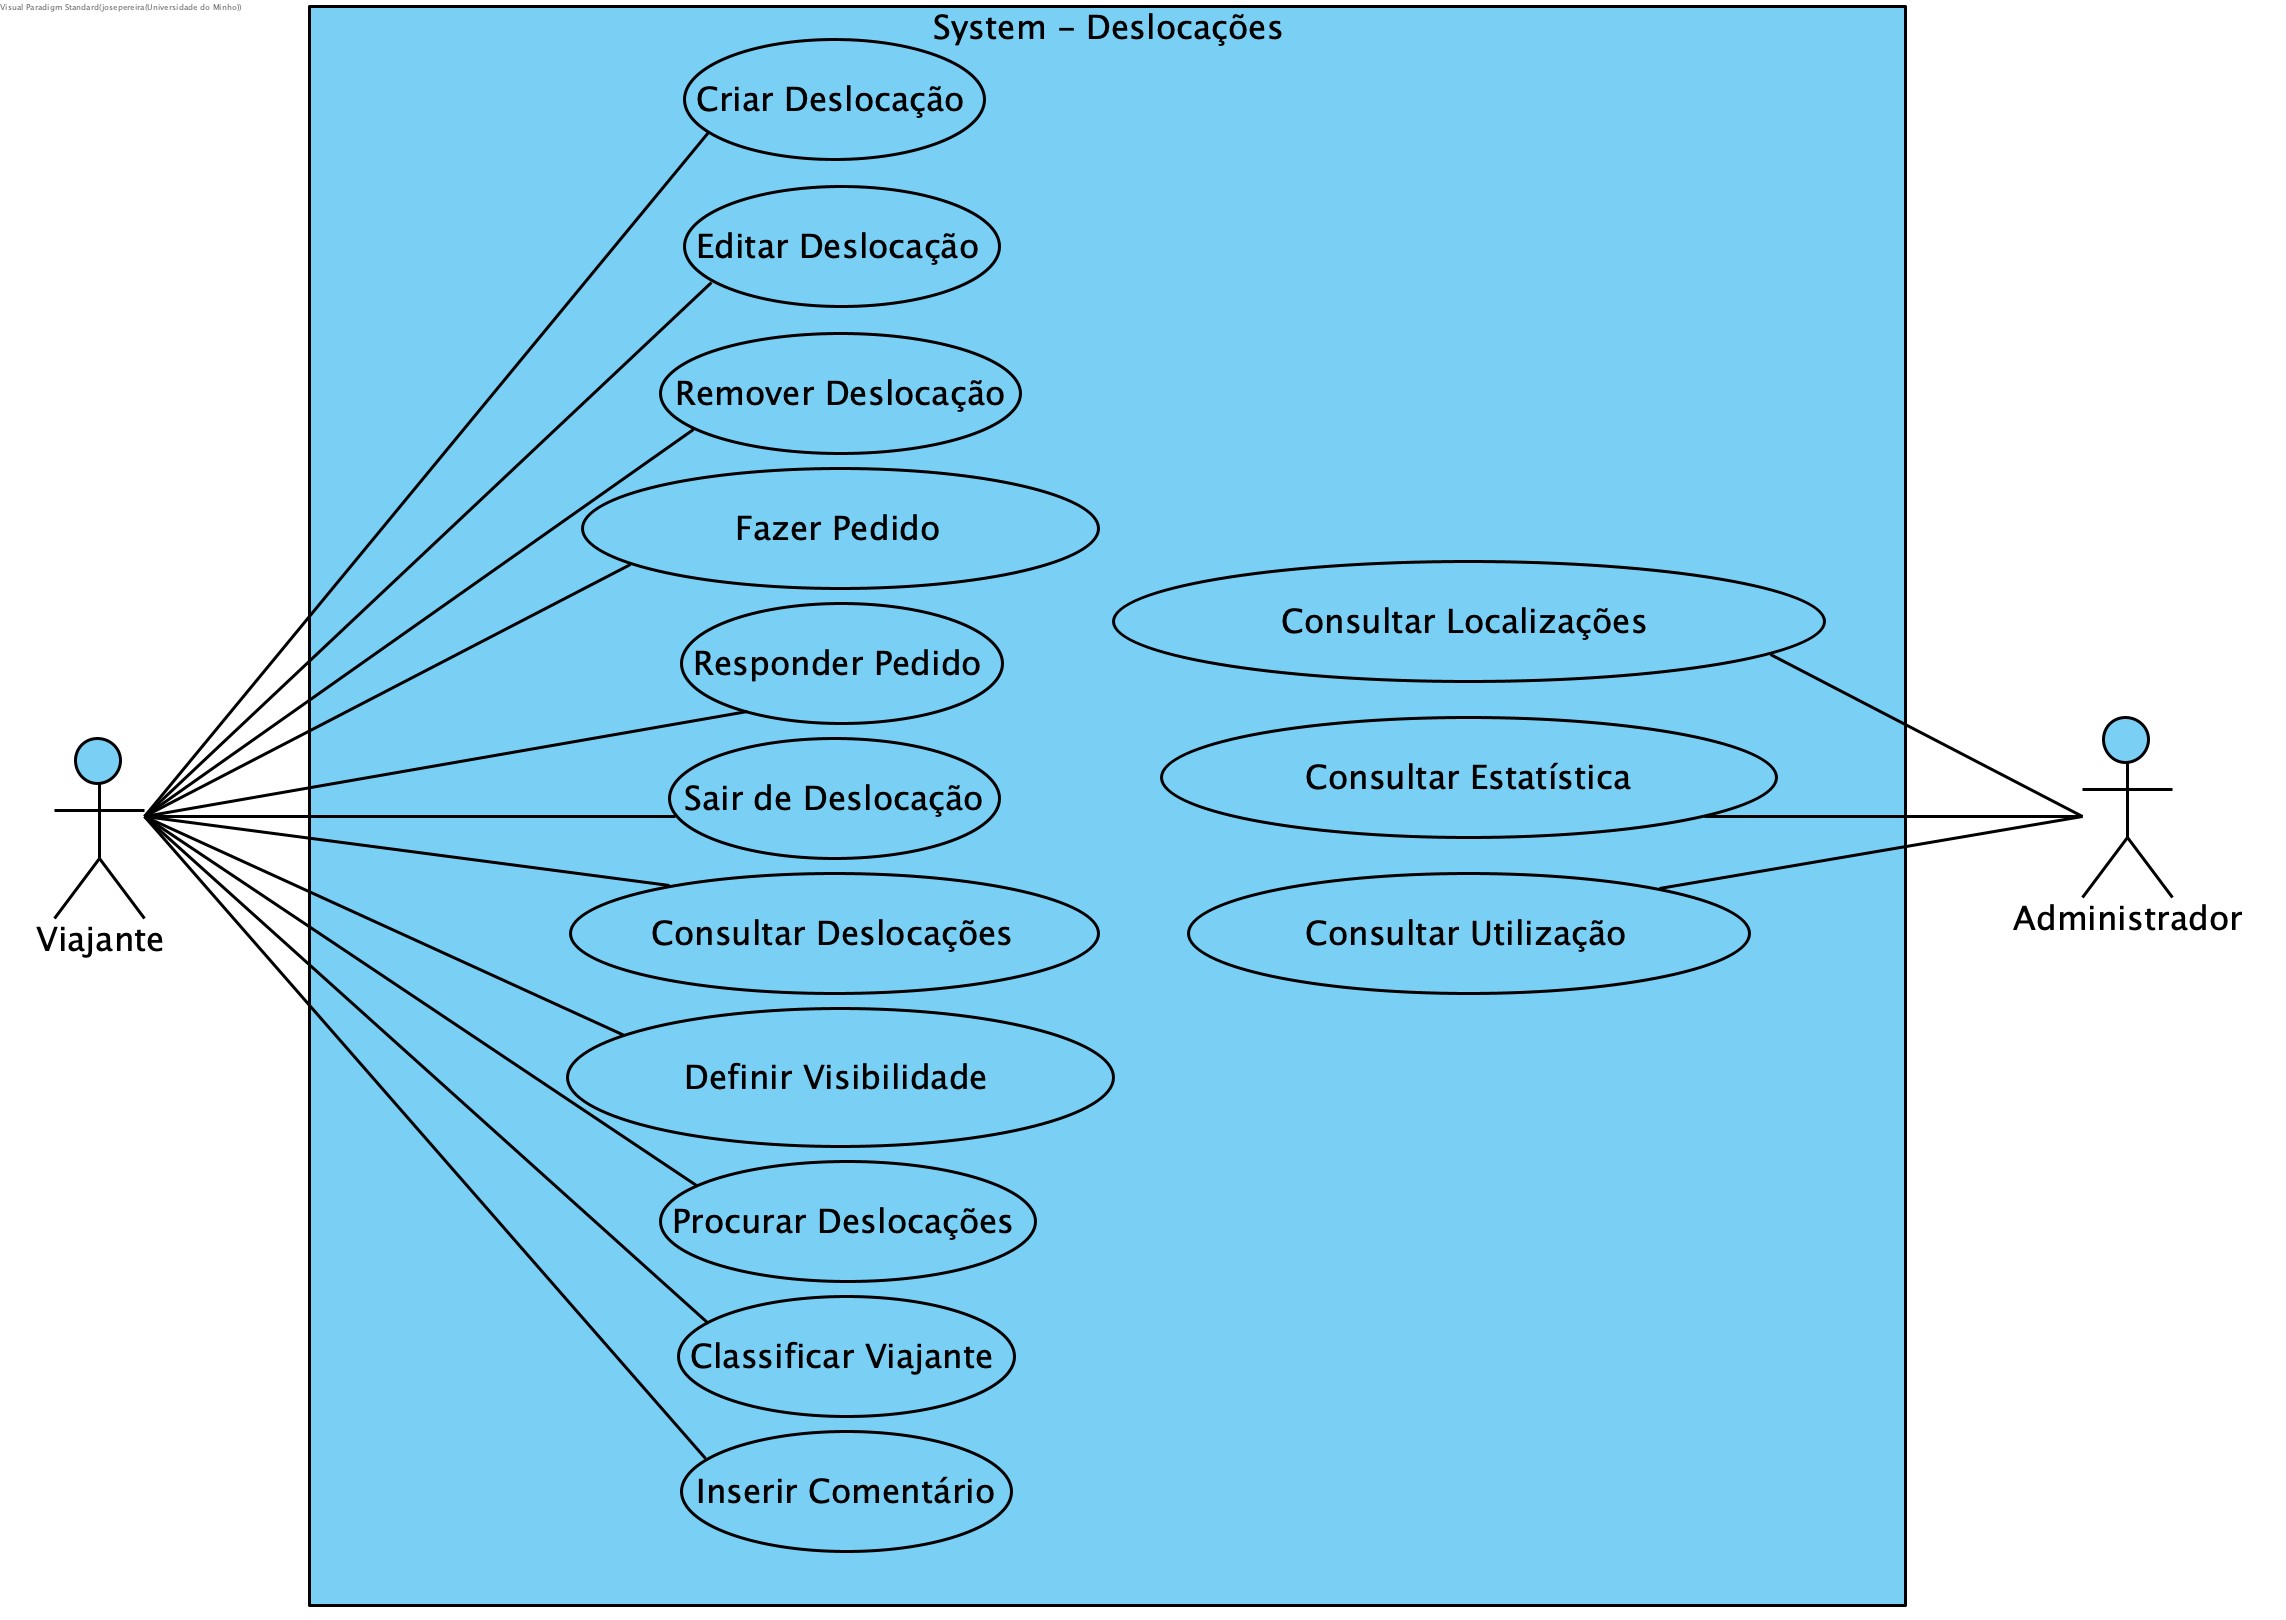
\includegraphics[scale=0.70]{imagens/diagrama-use-cases-2.png}
	\caption{Diagrama de Use cases.}
	\label{img:pag}
\end{figure}

\section{Respostas dos Inquéritos aos alunos da Universidade do Minho}

\begin{figure}[H]
    \centering
	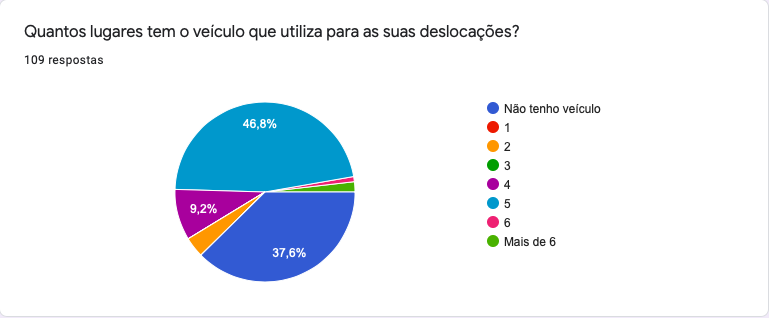
\includegraphics[scale=0.65]{imagens/i1.png}
	\label{img:pag}
\end{figure}

\begin{figure}[H]
    \centering
	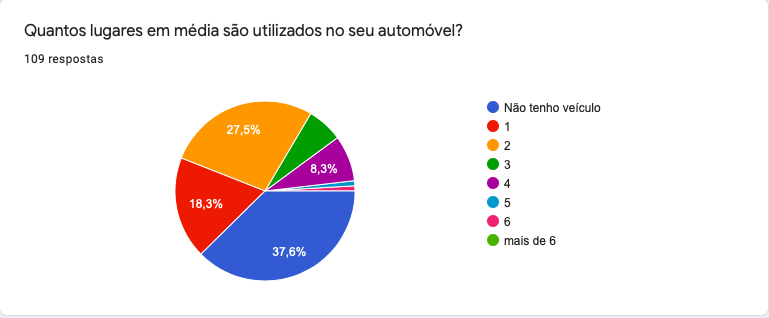
\includegraphics[scale=0.65]{imagens/i2.png}
	\label{img:pag}
\end{figure}

\begin{figure}[H]
    \centering
	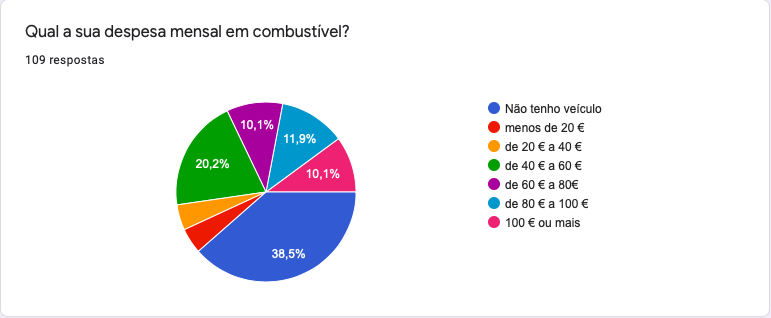
\includegraphics[scale=0.65]{imagens/i3.png}
	\label{img:pag}
\end{figure}

\begin{figure}[H]
    \centering
	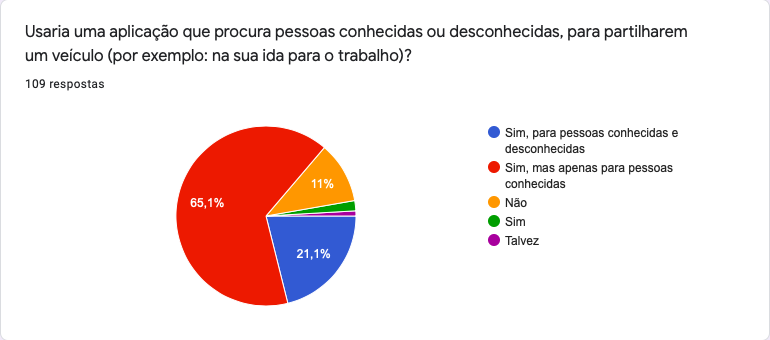
\includegraphics[scale=0.65]{imagens/i4.png}
	\label{img:pag}
\end{figure}

\begin{figure}[H]
    \centering
	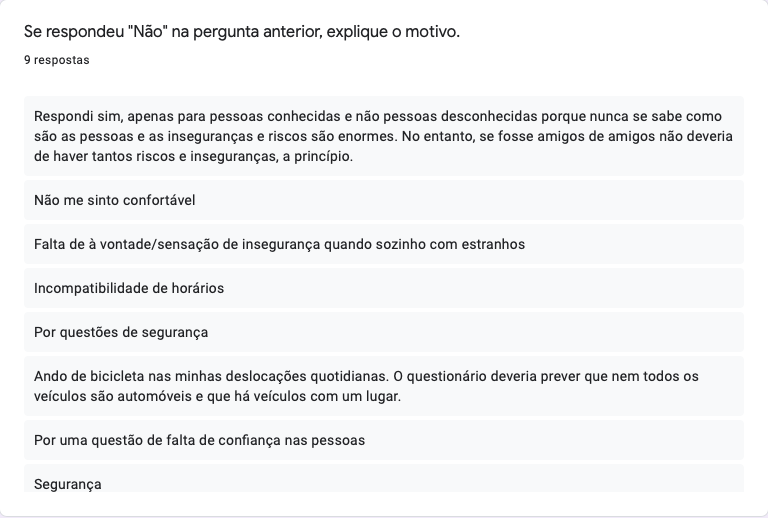
\includegraphics[scale=0.65]{imagens/i5.png}
	\label{img:pag}
\end{figure}



\end{document}
